\documentclass[manuscript,screen,nonacm]{sections/acmart}
\setcitestyle{numbers,sort&compress}
\settopmatter{printacmref=false}
\renewcommand\footnotetextcopyrightpermission[1]{}
\pagestyle{plain}

\usepackage{enumitem}
\usepackage{hyperref}
\usepackage{tabularx}
\usepackage{longtable}
\usepackage{pdflscape}
\usepackage{graphicx}
\usepackage{listings}
\usepackage{xcolor}
\usepackage{placeins}
\setlength{\textfloatsep}{8pt plus 2pt minus 2pt}
\setlength{\floatsep}{6pt plus 2pt minus 2pt}
\setlength{\intextsep}{6pt plus 2pt minus 2pt}
\captionsetup[figure]{skip=4pt, font=small}

\definecolor{codegreen}{rgb}{0,0.6,0}
\definecolor{codegray}{rgb}{0.5,0.5,0.5}
\definecolor{codepurple}{rgb}{0.58,0,0.82}
\definecolor{backcolour}{rgb}{0.95,0.95,0.92}

\lstdefinestyle{mystyle}{
    backgroundcolor=\color{backcolour},   
    commentstyle=\color{codegreen},
    keywordstyle=\color{magenta},
    numberstyle=\tiny\color{codegray},
    stringstyle=\color{codepurple},
    basicstyle=\ttfamily\footnotesize,
    breakatwhitespace=false,         
    breaklines=true,                 
    captionpos=b,                    
    keepspaces=true,                 
    numbers=left,                    
    numbersep=5pt,                  
    showspaces=false,                
    showstringspaces=false,
    showtabs=false,                  
    tabsize=2
}
\lstset{style=mystyle}

\title{Context-Aware Linguistic Steganography: A Generative Workflow using Large Language Models}

\author{Nasouh AlOlabi}
\affiliation{%
	\institution{Higher Institute for Applied Sciences and Technology}
	\city{Damascus}
	\country{Syria}}

\author{Riad Sonbol}
\affiliation{%
	\institution{Higher Institute for Applied Sciences and Technology}
	\city{Damascus}
	\country{Syria}}

\begin{document}

\begin{abstract}
	% Keep the abstract high-level: the detailed encode/decode workflow belongs in the main text,
% and this section should help future agents grasp the contribution quickly.
% Previous version kept here for reference:
% This paper proposes a context-aware \textbf{black-box} linguistic steganography workflow for threaded discussions that carries the payload through a \textit{selection channel} rather than token-level manipulation. The sender deterministically reconstructs a shared context corpus (post, comments, and topic-related domain documents), applies a payload transform and dictionary-based compression, and embeds bits in two layers: (i) selecting a reply parent in a deterministically flattened comment tree, and (ii) selecting an \textit{Angle} from a shared, deterministically generated angle set (category, source quote, tangent). A stochastic LLM then realizes the selected Angle as an ordinary visible reply; the visible text acts as a decodable witness of the selected Angle and does not rely on invisible or control characters. Before publishing, the sender runs a local decode simulation and retries synthesis until the intended Angle is recoverable or a retry budget is exhausted. The receiver locates the stego comment, reconstructs the pre-sender thread state under an agreed temporal window, regenerates the same angle set, and decodes the two selection indices to recover the payload. We report naturalness and distributional divergence (GPT-2 perplexity and word-unigram KL/JSD) on successful samples from clean run artifacts, and separate generation/decode failures from infrastructure errors.
This paper proposes a context-aware \textbf{black-box} linguistic steganography workflow for threaded discussions that carries the payload through a \textit{selection channel} rather than token-level manipulation. The sender reconstructs a shared context corpus, selects both a reply target and a semantic angle, and uses a stochastic LLM to realize the choice as an ordinary visible reply. The receiver rebuilds supplied pre-publication context and recovers the selected choices; exact recovery depends on shared operational parameters, synchronized inputs, and the supplied snapshot boundary. The method avoids invisible control characters, but does not claim token-level or information-theoretic security. We also document a historical audited configuration comparison: 554 of 627 project-side attempts succeeded, while the baseline lane was invoked on 460 attempts and accepted and decode-verified 304. Those artifacts used audit-assisted project-side recovery and reused source posts, so their capacity and quality differences are configuration-level evidence rather than a current, decision-grade superiority claim.

\end{abstract}

\keywords{Linguistic Steganography, Large Language Models, LLMs, Natural Language Processing, NLP, Black-box Steganography, Semantic Embedding, Agentic Workflows, Imperceptibility}

\maketitle

\section{Introduction}
\label{sec:introduction}

Linguistic steganography hides a secret inside ordinary text.
Early methods mostly swapped synonyms \cite{qiang2023natural}.
Natural language has little spare room, so even small statistical quirks can give a detector something to grab \cite{yang2020vae,kaptchuk2021meteor,Wang_2023}.
Large language models changed the cover: instead of editing an existing sentence, many systems now generate the text \cite{li2023rewriting,lin2024zero,wu2024generative}.
Those systems usually hide bits by steering next-token sampling, which can look fluent while still sitting on a modified distribution.

However, existing LLM-based steganographic systems remain constrained by a fundamental trade-off between statistical security and perceptual naturalness \cite{lin2024zero,wu2024generative,li2023rewriting}. While a model may output grammatically and statistically fluent sentences, these often lack the deep semantic coherence required for specific communicative contexts, such as threaded social media discussions \cite{liao2024co,wang2023hi,zhang2024controllable}. A comment that is fluent but off-topic is conspicuous to a human reader and to a semantic checker.

We hide the payload in two conversational choices rather than in token probabilities.
Bits select (i) which comment to reply to in a depth-first flattened thread, and (ii) which \textit{Angle} to talk about from a list both parties rebuild from the public thread and a shared research procedure.
A language model then writes an ordinary visible reply for that pair.
We do not use invisible characters.
Before the comment is kept, the sender runs the same Angle decoder the receiver will use and retries if that decode misses.
Figure~\ref{fig:token-vs-intent} contrasts token-level embedding with this two-layer selection channel.
% ------------------------------------------------------------------
% AI IMAGE PROMPT (fig:token-vs-intent) -> figures/token_vs_intent_embedding.(png|pdf)
% ------------------------------------------------------------------
% GLOBAL STYLE: Academic technical diagram, flat vector infographic, 16:9 or 2:1 landscape,
%   300 DPI target, white or #F8FAFC background, high contrast, sans-serif labels (simulate
%   Helvetica / Inter), slate blue #334155 primary, teal #0D9488 secondary, amber #D97706
%   accents, thin 1--2pt strokes, optional subtle card shadows. No photorealistic humans,
%   no Reddit Snoo or brand logos, no watermarks, no 3D renders, no cluttered stock icons.
% COMPOSITION: Three-column layout. Vertical divider lines or generous whitespace between
%   columns. Top centered small title: "Embedding domain: token vs communicative intent".
% LEFT PANEL (width ~38%): Header bar "Token / distribution embedding (typical)".
%   Below: horizontal row of 8--12 small rectangles as fake tokens (single letters or
%   [tok] placeholders). Arrow down to a stacked bar or histogram labeled "next-token
%   distribution / logits". Second arrow to a die or branching arrows labeled "sampling".
%   Small triangular warning badge with text "often needs white-box logits" and sublabel
%   "fragile in threaded social context". Use cool gray tones; keep diagram busy but legible.
% CENTER (~12%): Large vertical double chevron or bold arrow pointing upward, label
%   "shift to semantic layer" on two lines, color teal.
% RIGHT PANEL (~38%): Header "Semantic / intent embedding (this work)". Generic forum UI:
%   rounded rectangle "Original post" at top; 2--3 nested "Comment" cards with indent guides;
%   one comment node outlined in amber with pin icon, label "Layer 1: reply target".
%   From that node, fan out 4--6 small rounded chips labeled "Angle 0..N" (Layer 2).
%   One chip highlighted; arrow to final speech bubble "Stego reply (cover text)".
%   Optional tiny caption strip: "Shared deterministic reconstruction (thread + research)".
% LEGIBILITY: All English labels at least 8pt equivalent when scaled to single-column
%   figure width in ACM manuscript. Avoid micro-font paragraphs; use short phrases only.
% NEGATIVE PROMPT: blurry text, illegible handwriting, isometric clutter, cyberpunk neon,
%   anime, screenshots of real apps, dense equations, more than two sentences of body text.
% ------------------------------------------------------------------

\begin{figure}[t]
	\centering
	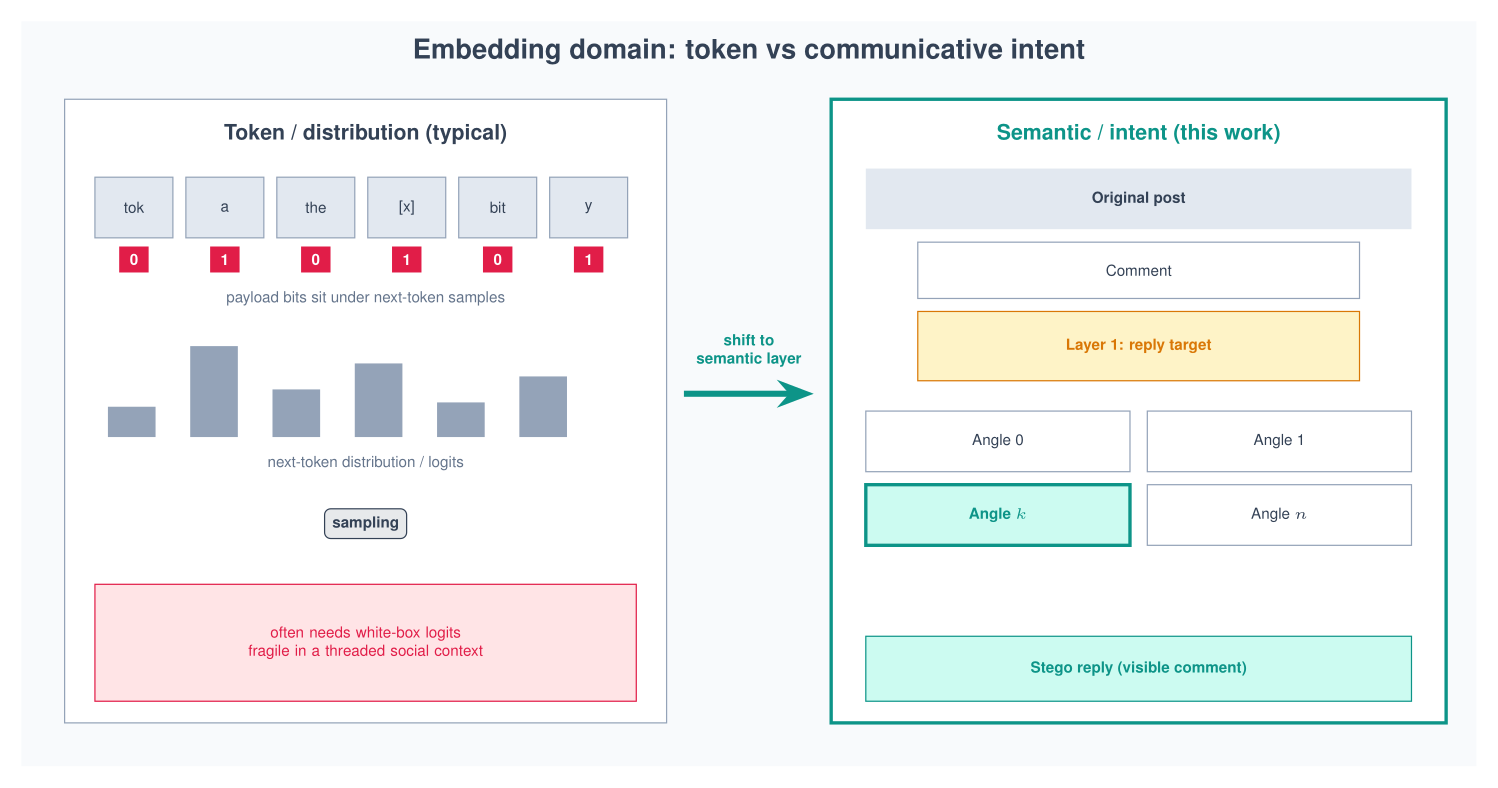
\includegraphics[width=0.78\linewidth]{figures/token_vs_intent_embedding}
	\Description{Side-by-side contrast: token-level steganography versus two-layer semantic embedding (reply placement and thematic intent) in a discussion thread.}
	\caption{Conceptual contrast between token-level embedding and our two-layer semantic embedding over a threaded discussion.}
	\label{fig:token-vs-intent}
\end{figure}

The primary contributions of this paper are:
\begin{itemize}
    \item A two-layer, selection-channel embedding architecture for threaded discussions that encodes bits into reply targeting and Angle selection, with a visible reply rather than a hidden carrier.
    \item A reconstruction pipeline (thread plus reproducible research) that does not need white-box logits. Reported payload recovery still uses sender-side audit metadata.
    \item A closed-loop verification mechanism that simulates decoding before the comment is kept and retries synthesis, with an optional revision pass, under stochastic generation.
    \item An independent LLM-judge comparison on 244 unique-output pairs against the official ZLG baseline, reported together with source-run reliability and a historical 304-pair configuration table, with explicit denominators and without a superiority claim.
\end{itemize}

\section{Background}
\label{sec:background}

Among the classical concerns of information security---protecting content through encryption, preserving user privacy, and concealing the existence of communication itself---this work is concerned with the last. \textbf{Steganography} differs from encryption in a fundamental way: rather than making a message unreadable, it makes the message invisible by embedding it inside an ordinary carrier, such as an image or a piece of text, so that an observer has no reason to suspect anything is hidden. \textbf{Imperceptibility} is therefore the primary objective, not confidentiality per se.

Text is a particularly challenging carrier due to its low redundancy and strict semantic constraints. The classical ``Prisoners' Problem'' \cite{simmons1984prisoners} illustrates the goal: two parties, Alice and Bob, must exchange hidden information without alerting a watchful adversary.

Textual steganography methods are typically divided into \textbf{format-based} approaches, which exploit layout or structural features, and \textbf{linguistic-based} approaches, which modify linguistic form. Within the latter, early techniques such as \textbf{synonym substitution} embed bits by altering lexical choices, but suffer from low capacity and high detectability.

More formally, generative linguistic steganography operates through an \textbf{embedding function} $f_{emb}$ that establishes a cryptographic and linguistic mapping to hide secret messages within generated text. The algorithm takes as inputs a language model $\mathcal{L}$ and a secret message $m$ (represented as a uniformly distributed bitstream). At each generation step, rather than sampling freely from the language model's conditional distribution $p_{LM}$, the embedding function $f_{emb}$ \textbf{restricts or modifies} the token selection process according to the message bits being embedded. This specialized process is known as \textbf{steganographic sampling}, producing a steganographic text (stegotext) $y$. The security of the system depends on minimizing the divergence between the original language model distribution $p_{LM}$ and the modified distribution $q$ induced by $f_{emb}$ \cite{zhang2021provably}.

Traditional linguistic approaches offer limited embedding capacity and often leave statistical artifacts. Advances in deep learning and \textbf{Large Language Models (LLMs)} now enable generative methods that achieve higher text quality and more secure embedding. Evaluating such systems requires several dimensions of imperceptibility: \textbf{perceptual} (human naturalness), \textbf{statistical} (distributional similarity to natural text), and \textbf{cognitive} (semantic and contextual fidelity) \cite{ding2023context}.

LLM use in steganography also introduces new sources of detectability. \textbf{Hallucination}---where a model generates content that is factually unsupported, semantically inconsistent, or poorly grounded in the preceding context---is one such source. In ordinary text generation, hallucination is mainly a reliability concern. In steganographic generation, it becomes a security concern as well: even a fluent sentence can expose a hidden channel if it contains an unsupported claim, an abrupt topic shift, or a contradiction with the surrounding context. Hallucination therefore threatens \textbf{cognitive imperceptibility}, since generated text must remain contextually plausible and communicatively coherent, not merely surface-fluent.

Distinct from hallucination, the \textbf{PSIC effect} (Perceptual-Statistical Imperceptibility Conflict) \cite{yang2020vae} captures a different and arguably more fundamental tension in generative linguistic steganography. Text that is optimized for human fluency is not necessarily statistically indistinguishable from natural human text. For example, selecting only high-probability tokens can produce sentences with low perplexity and strong local readability, but it may also make the generated distribution overly smooth, regular, or concentrated compared with real human writing. Such text can appear natural to readers while remaining detectable to statistical steganalyzers \cite{yang2020vae}.

The PSIC effect therefore shows that \textbf{perceptual imperceptibility} and \textbf{statistical imperceptibility} are related but not identical goals. Human-written text often contains variation, irregularity, and locally unexpected word choices. By contrast, overly fluent model-generated text may lack this natural variance. Increasing the embedding rate can sometimes force the sampler to select from a broader range of tokens, which may better approximate the diversity of human text; however, this same process can also reduce readability or semantic coherence if the token choices become poorly aligned with the context. Thus, higher capacity does not automatically imply better security. Secure generative steganography requires balancing embedding rate, fluency, distributional similarity, and contextual consistency.

\subsection{Large Language Models as Text Generators}
\label{sec:background-llm-generators}

Large Language Models (LLMs) are autoregressive, generative systems based on the Transformer architecture \cite{vaswani2017attention} that approximate high-dimensional distributions over natural-language sequences \cite{kaptchuk2021meteor,radford2019language}. Given a prefix, an LLM emits a probability vector over the vocabulary; the next token is sampled from this vector and appended to the prefix, and the process repeats until a stopping criterion is met. During pre-training, billions of parameters are tuned on large text corpora so that the model's predictive distribution approximates patterns in the training data \cite{brown2020language}. As a consequence, modern LLMs can produce text with high fluency, coherence, and stylistic control \cite{bubeck2023sparks}. The learned representations capture stylistic and semantic regularities that generalize across domains, enabling applications requiring nuanced linguistic mimicry \cite{reif2022recipe}.

\subsection{Large Language Models in Generative Linguistic Steganography}
\label{sec:background-llm-stego}

Because text produced by modern LLMs can closely resemble ordinary human-authored text, these models provide effective engines for generative text steganography. Rather than editing an existing cover, a growing line of work treats the model itself as a steganographic sampler: the hidden message steers generation, so the stego text is drawn from a realistic communication distribution from the start. The public availability of high-quality models, together with the efficiency of sampling-based embedding, has made this route more practical than earlier designs.

LLMs like \textbf{GPT-2} \cite{radford2019language}, \textbf{LLaMA} \cite{touvron2023llama2}, and \textbf{Baichuan2} \cite{yang2023baichuan2} are commonly used as basic generative models for steganography. Most such schemes couple the language model with a steganographic code that ties message bits to token choices: at each generation step, the bits to be hidden determine which candidate token is emitted from the model's next-token distribution. However, traditional ``white-box'' methods necessitate sharing the exact language model and training vocabulary, which limits fluency, logic, and diversity compared to texts generated by modern black-box LLM APIs. These methods inevitably alter sampling probability distributions when embedding messages, posing security risks \cite{wu2024generative}. \textbf{Black-box approaches} avoid these limitations by leveraging state-of-the-art hosted models to deliver better text quality, faster generation speeds, and minimal local resource requirements. However, this paradigm trades fine-grained control over internal sampling for these practical advantages. Conversely, \textbf{white-box access} enables precise parameter control and stronger security guarantees, but demands substantial computational resources, engineering effort, and higher latency---raising deployment barriers. This trade-off between access paradigms is central to evaluating the robustness and applicability of modern linguistic steganography, and it directly motivates the black-box design adopted in Section~\ref{sec:methodology}.

New approaches, such as \textbf{LLM-Stega} \cite{wu2024generative}, explore black-box generative text steganography using the user interfaces (UIs) of LLMs, which removes any need to observe internal sampling distributions. Secret bits are encrypted and mapped onto a prearranged keyword set that steers generation, and candidate outputs from which the message cannot be recovered are discarded via reject sampling, preserving both extraction accuracy and semantic quality \cite{wu2024generative}.

Another framework, \textbf{Co-Stega}, leverages LLMs to address the challenge of low capacity in social media. It expands the space available for hiding messages through context retrieval and uses purpose-built prompts to raise the entropy of the generated replies, which in turn enlarges the embedding capacity while keeping the output fluent and topically relevant \cite{liao2024co}.

\textbf{Zero-shot linguistic steganography} instead relies on in-context learning: covertext samples are supplied in the prompt, and the stego text is produced within a question--answer (QA) exchange, so the output reads as a natural reply rather than as free-standing generated text \cite{lin2024zero}.

The increasing popularity of deep generative models has made it feasible for provably secure steganography to be applied in real-world scenarios, as they fulfill requirements for perfect samplers and explicit data distributions \cite{ding2023discop, kaptchuk2021meteor, qi2024provably}.

LLM-based steganographic methods are typically evaluated on two primary axes: imperceptibility (perceptual, statistical, and cognitive measures) and embedding capacity (e.g., bits per token or bits per word). Imperceptibility evaluations may include automatic metrics (PPL, Distinct-n, KL/JSD) as well as human judgements; embedding capacity is usually reported as bits/token or overall embedding rate. Section~\ref{sec:related_work} surveys how the literature applies, evaluates, and constrains these methods in more detail.

\section{Methodology}
\label{sec:methodology}

We propose a black-box steganographic method that hides a secret message inside a public conversation.
The sender and the receiver both have accounts on a social media platform.
The sender finds a thread, writes what looks like a normal comment or reply, and publishes it.
The receiver later reads that same thread, finds the sender's contribution, and recovers the hidden payload.
Our study uses Reddit-style data as the main case.
The design targets any threaded discussion environment; whether it transfers cleanly to other platforms remains to be evaluated.
Figure~\ref{fig:end-to-end} shows the end-to-end covert scenario and the shared assumptions needed for synchronization.
%
% ------------------------------------------------------------------
% AI IMAGE PROMPT (fig:end-to-end) -> figures/end_to_end_scenario.(png|pdf)
% ------------------------------------------------------------------
% GLOBAL STYLE: Flat vector flowchart, landscape, generous margins, same paper color system.
% LEFT THIRD: Rounded card "Alice / sender agent" with minimal laptop or terminal icon
%   (geometric, not Apple logo). Small bullet trio: "encode", "verify", "publish".
% CENTER: Vertical stack of three rounded rectangles mimicking a thread: wide "Post",
%   indented "Comment thread", indented "Reply chain (selected parent)". Banner above stack:
%   "Public threaded forum (e.g., Reddit-style)". No brand marks.
% RIGHT THIRD: Card "Bob / receiver agent" with eye-on-thread or inbox icon; labels
%   "snapshot + filter by T_sync", "decode payload".
% ARROWS: Alice -> center: "posts stego-comment". Center -> Bob: "reads public thread".
% SHARED SECRETS BAND (below center or in lower third): Two lock-and-key or keyhole icons
%   in a horizontal row. (1) Label: "Shared: deterministic preprocessing + identical LLM (T=0)
%   for angle reconstruction". (2) Label: "Agreed temporal window T_sync". Use monospace only
%   for T_sync and T=0 if needed.
% ADVERSARY (optional, far edge): Faint gray silhouette "Passive observer" with "?"
%   and caption "does not share secret parameters" to stress black-box sync, not crypto keys
%   to the platform.
% LEGIBILITY: Single-page story; avoid crossing arrows; orthogonal routing preferred.
% NEGATIVE PROMPT: network topology maps, OSI stack, encryption shields only, real Reddit UI,
%   QR codes, binary matrix rain.
% ------------------------------------------------------------------

\begin{figure}[t]
	\centering
	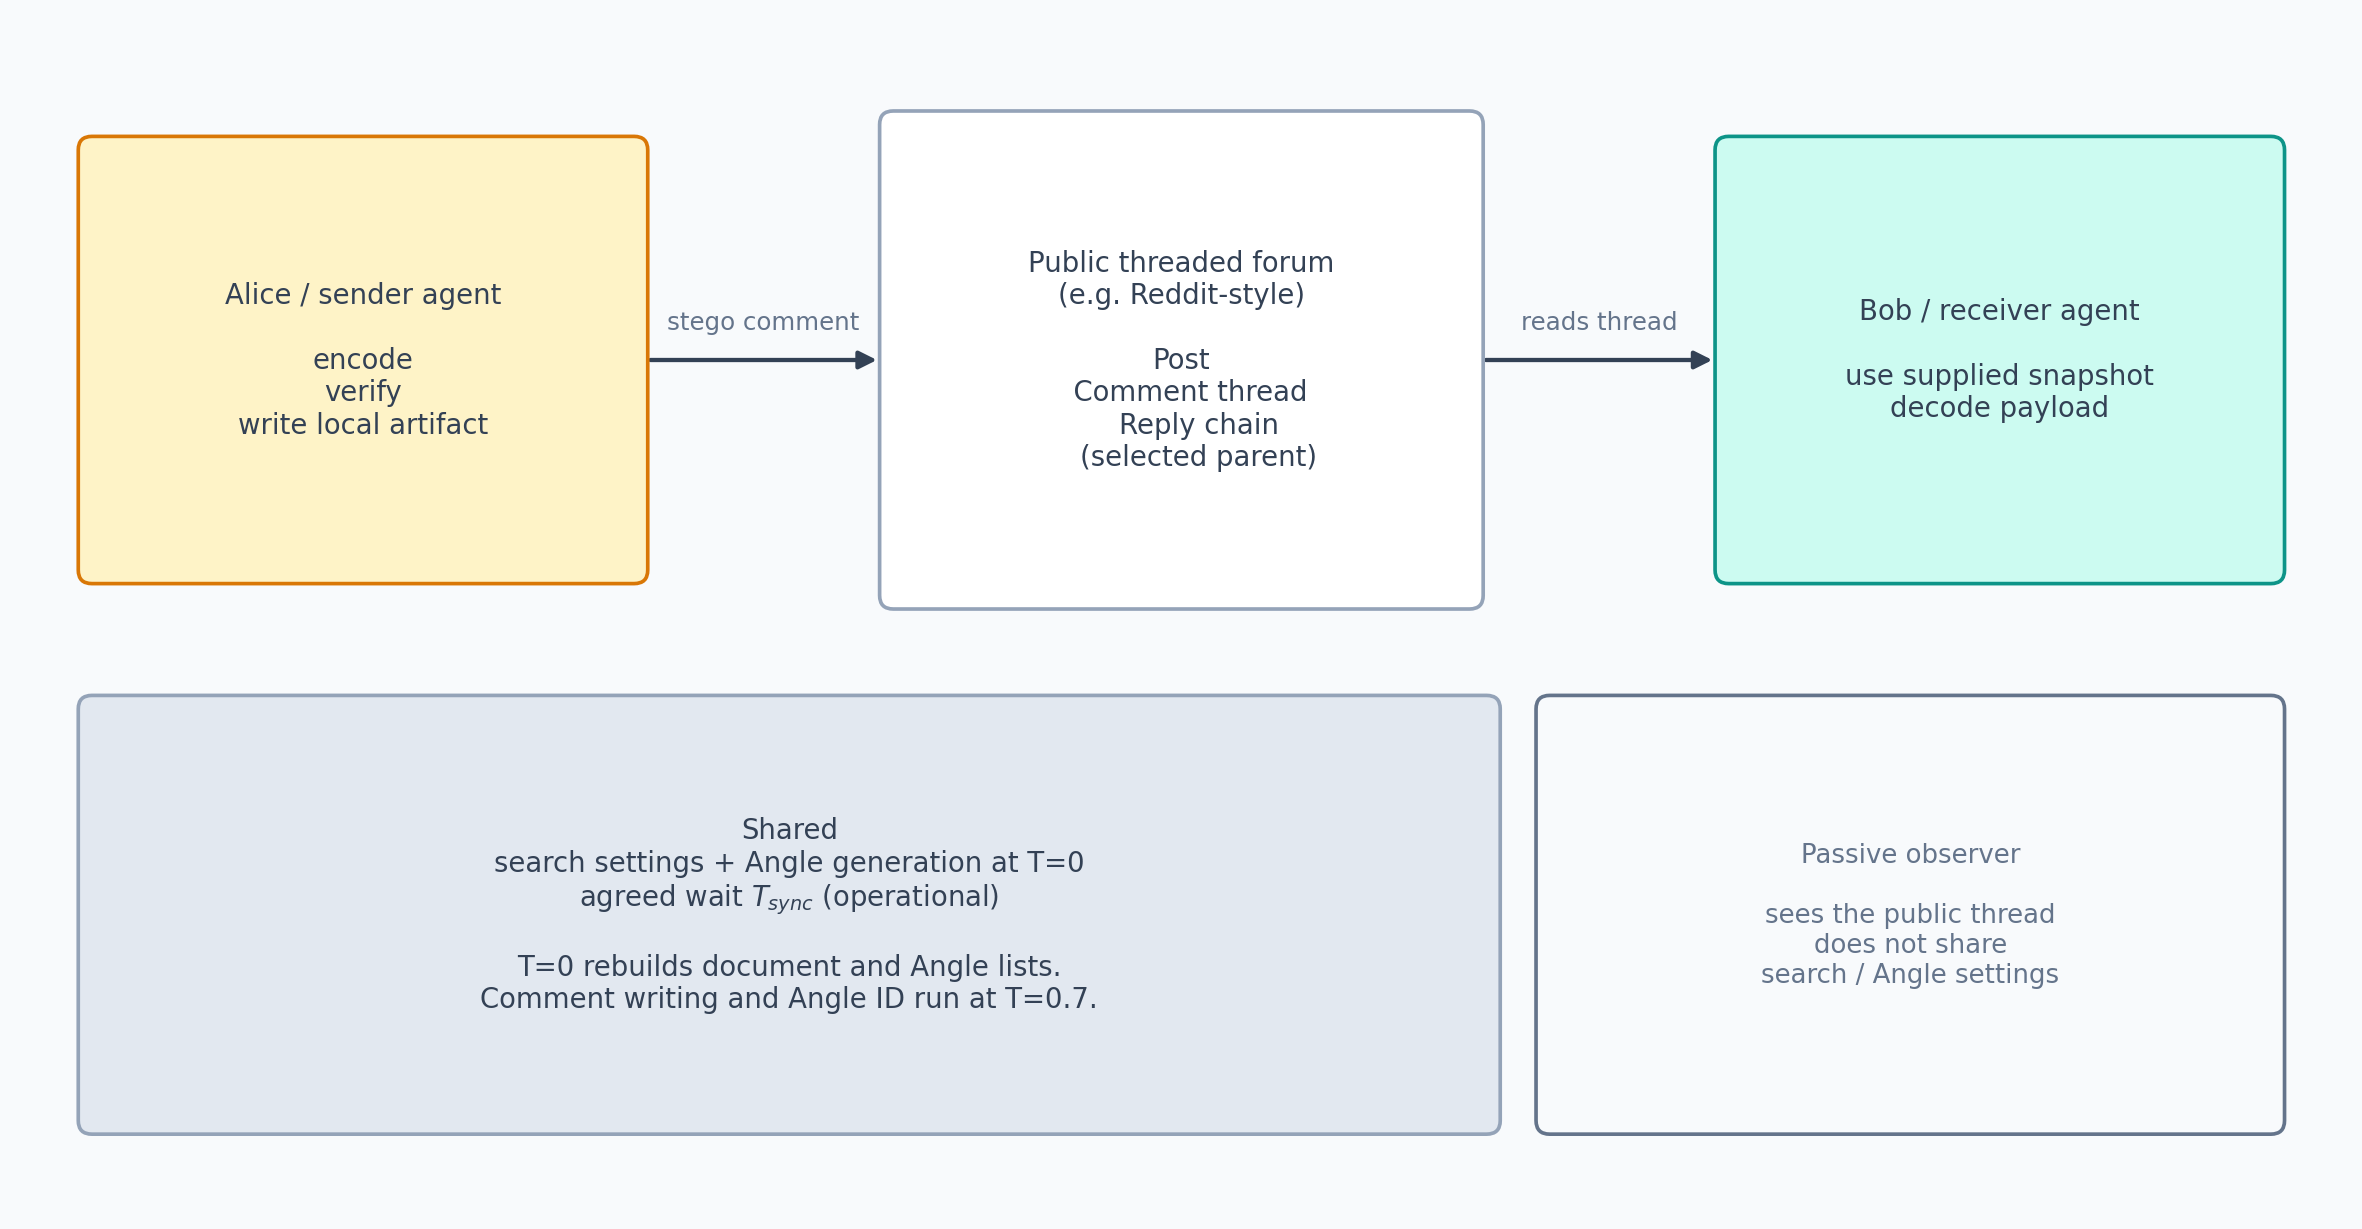
\includegraphics[width=0.78\linewidth]{figures/end_to_end_scenario.png}
	\Description{Diagram of Alice and Bob communicating covertly over a public threaded forum: sender encodes and publishes a reply; receiver snapshots the thread using an agreed time window and shared operational parameters.}
	\caption{Covert communication scenario: Alice and Bob use a public threaded channel; synchronization relies on shared operational parameters and a negotiated temporal window.}
	\label{fig:end-to-end}
\end{figure}

\subsection{System Architecture}
The core of the proposed framework centers on a multi-layer embedding process that leverages both the \textit{spatial location} of the response and the \textit{thematic subject} of the content as carriers for the secret payload. By mapping binary data to high-level conversational actions---specifically, the selection of a reply target and the selection of an \textit{Angle}---the system carries the payload through a selection channel while preserving perceptual naturalness in the visible text. In the implemented workflow, the receiver reconstructs the same pre-sender context (thread snapshot + deterministic research + regenerated angles) and decodes the same selection indices to recover the payload. Figure~\ref{fig:two-layer} depicts the two embedding layers and their interaction with synthesis.

\subsection{Operational Requirements}
To achieve synchronization, both the sender and receiver must maintain access to:
\begin{itemize}
    \item \textbf{Public Communication Channel:} Accounts on the target social media platform.
    \item \textbf{Shared Operational Parameters:} A deterministic search algorithm, post metadata, and predefined search constraints.
    \item \textbf{Deterministic Reconstruction Settings:} A synchronized model/backend configuration for deterministic stages (e.g., \texttt{temperature=0}) so both parties regenerate the same search terms and angle set from the same inputs.
    \item \textbf{Agreed Temporal Window:} A negotiated $T_{sync}$ used to filter thread state so the receiver reconstructs the same parent-comment context seen by the sender.
\end{itemize}

\subsection{Search Determinism \& Synchronization Framework}
\label{sec:search_determinism}
Ensuring that both Alice and Bob operate on the same researched corpus is the cornerstone of reliable decoding. The implemented research stage is a reproducible preprocessing chain rather than an ad hoc web search. A search-term generator first extracts 12--20 unique queries from the post title, body, and URL using the workflow LLM at \texttt{temperature=0}. Each query is then executed through the Google Custom Search backend with a fixed request shape (\texttt{first=1}, \texttt{count=10}), duplicate links and PDF results are removed, and the surviving URLs are fetched in batches of three. Content extraction uses a crawl4ai-based adapter that normalizes URLs and extracts the primary text content. The resulting flat list of fetched page texts is stored as a search-results corpus, and the pipeline records term and corpus integrity hashes so the same corpus can be replayed by downstream stages. Figure~\ref{fig:research-pipeline} summarizes this deterministic research chain.
% 
% ------------------------------------------------------------------
% AI IMAGE PROMPT (fig:research-pipeline) -> figures/research_pipeline_deterministic.(png|pdf)
% ------------------------------------------------------------------
% FORMAT: Extra-wide landscape (approx 3:1 or 16:5) for figure* / full text width.
% STRUCTURE: Single horizontal pipeline of FIVE rounded rectangles, equal height, left-to-right
%   arrows with arrowheads. Number each box small "1".."5" in corner.
% BOX 1: "Source Inputs". Icon: document stack. Labels: "Post title, body, URL", "Top comments".
% BOX 2: "Search-Term Generator". Icon: AI chip. Subtext: "LLM (T=0) -> 12--20 queries".
% BOX 3: "Fixed-Shape Search". Icon: magnifying glass over list. Label: "Google Search API".
%   Micro-label: "first=1, count=10" (monospace).
% BOX 4: "Filtering & Extraction". Icon: filter funnel. Labels: "Drop PDFs", "Dedup links",
%   "Batched fetch (3)".
% BOX 5: "Deterministic Corpus". Icon: stack of papers. Hash badges: "search term hash",
%   "search results hash".
% FOOTER: Centered small caption strip "Reproducible preprocessing chain (Alice == Bob)".
% COLOR: Alternate box fill white vs very light blue-gray; connectors dark slate.
% NEGATIVE PROMPT: database icons, cylinders, server racks, Google logo, messy wireshark,
%   chaotic arrows, illegible hash strings longer than 16 chars.
% ------------------------------------------------------------------

\begin{figure*}[t]
	\centering
	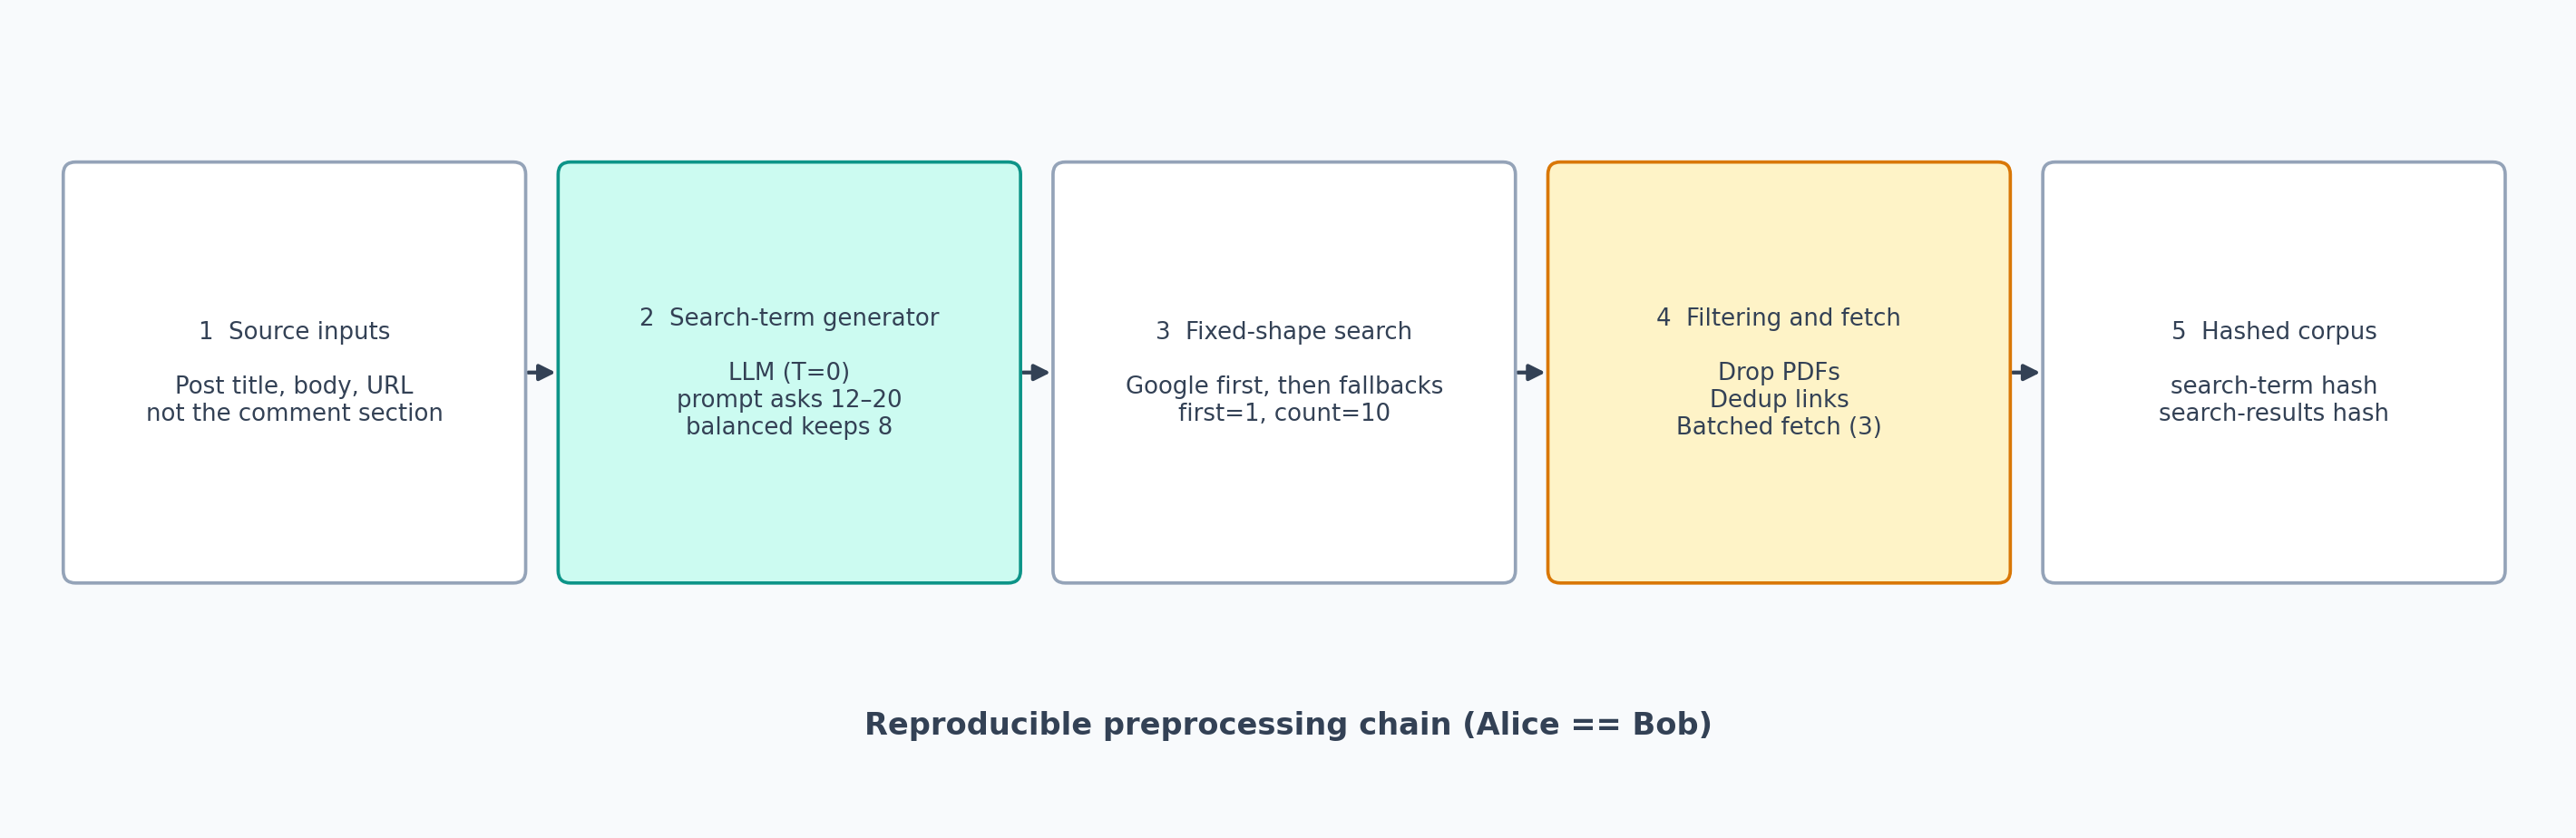
\includegraphics[width=\textwidth,height=0.62\textheight,keepaspectratio]{figures/research_pipeline_deterministic}
	\Description{Horizontal pipeline from source inputs through deterministic search-term generation, fixed-shape search API, filtering and fetching, to a hashed search-results corpus for reproducibility.}
	\caption{Deterministic research stage: shared term generation, fixed search parameters, filtering, batched fetching, and integrity hashes for replayable corpora.}
	\label{fig:research-pipeline}
\end{figure*}

\subsection{State Synchronization (Temporal Window)}
To ensure that both Alice and Bob visualize an identical state of the conversation tree, they must adhere to a negotiated \textit{Temporal Window Duration} ($T_{sync}$). This synchronization mechanism is operationalized to address the processing latency inherent in the sender's agent:
\begin{enumerate}
    \item \textbf{Sender Side:} Alice captures a snapshot of the discussion thread at time $t_{start}$, performs the multi-layer embedding, and subsequently publishes the generated stego-comment at $t_{publish}$.
    \item \textbf{Receiver Side:} Upon identifying the stego-contribution published at $t_{publish}$, Bob filters the thread's historical state to include only those comments established prior to $t_{publish} - T_{sync}$.
\end{enumerate}
The agreed-upon duration $T_{sync}$ is an external synchronization requirement: the receiver must supply a pre-publication snapshot or apply the timestamp cutoff before reconstruction. The current receiver removes the sender comment and rebuilds from the supplied post, but does not itself enforce this timestamp cutoff; enforcement is an operational responsibility of the caller or acquisition layer. Figure~\ref{fig:tsync} shows the intended temporal window relative to $t_{start}$ and $t_{publish}$.
%
% ------------------------------------------------------------------
% AI IMAGE PROMPT (fig:tsync) -> figures/temporal_sync_window.(png|pdf)
% ------------------------------------------------------------------
% TYPE: Single horizontal timeline diagram, landscape, plenty of vertical space for brackets.
% MAIN AXIS: Thick horizontal line with tick marks; left label "thread history ->", right
%   "later". Use subtle gray grid optional.
% MARKERS ON AXIS: (a) Camera or snapshot icon at t_start with label "t_start: Alice snapshots
%   thread". (b) Shaded band from t_start to t_publish (light amber fill) labeled
%   "Sender pipeline (embedding + synthesis latency)". (c) Upload / paper-plane icon at
%   t_publish labeled "t_publish: stego comment appears".
% BOB'S CUTOFF: Below the axis, a horizontal curly brace or square bracket spanning from
%   "thread beginning" (or earliest comment icon) to the point (t_publish - T_sync). Label:
%   "Bob includes comments with time <= t_publish - T_sync". Typeset T_sync with subscript
%   style if possible.
% CONFLICT EXAMPLE: One or two small comment dots AFTER the cutoff vertical line; color red
%   or hatched overlay, label "excluded: arrived during Alice's run". Legend box lower corner
%   with swatch explanations.
% RATIONALE MICROTEXT (one line): "Agreed T_sync prevents parent-comment mismatch".
% NEGATIVE PROMPT: Gantt chart software screenshot, clock faces everywhere, time zones map,
%   relativity diagrams.
% ------------------------------------------------------------------

\begin{figure*}[t]
	\centering
	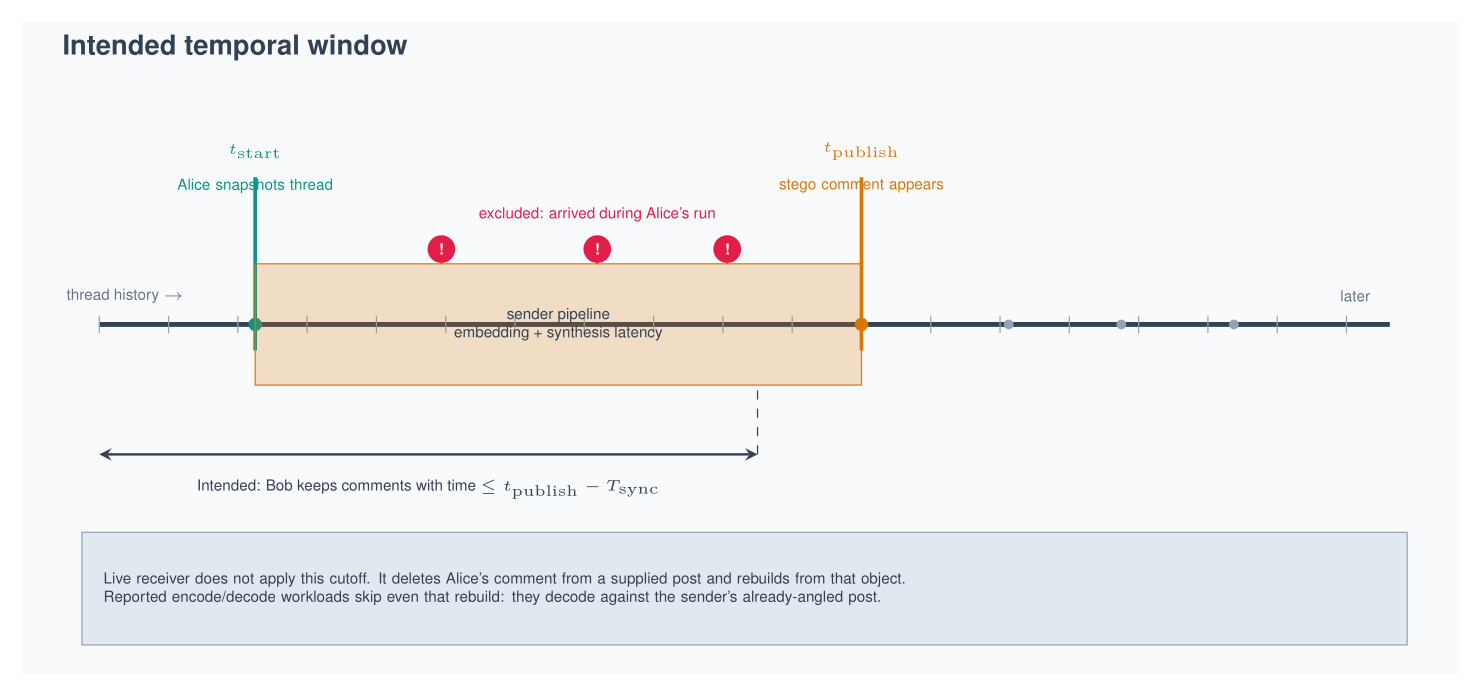
\includegraphics[width=\textwidth,height=0.58\textheight,keepaspectratio]{figures/temporal_sync_window}
	\Description{Timeline diagram showing comment inclusion cutoff at publish time minus an agreed synchronization window, excluding comments that arrive while the sender is still working.}
	\caption{Temporal synchronization: Bob's reconstructed thread state matches Alice's by agreeing on $T_{sync}$ and filtering comments relative to $t_{publish}$.}
	\label{fig:tsync}
\end{figure*}

\subsection{Payload Preparation \& Compression}
\label{sec:compression}
Before embedding, the payload passes through two reversible stages: an optional protection transform, then a dictionary-based compressor. Both stages are implemented once, in a single codec module that the sender and receiver both call directly --- not two separate copies that could drift apart. Everything above that module (the sender and receiver pipelines) is limited to I/O, caching, and orchestration.

\subsubsection{Protection Transform}
The transform is chosen by configuration and recorded in the sender audit, so the receiver knows which inverse to apply. Three modes are implemented:
\begin{itemize}[leftmargin=*]
    \item \texttt{plain} (default): the payload is passed through unchanged.
    \item \texttt{hmac\_xor\_v1}: a keystream cipher. A fresh 16-byte nonce $N$ and a pre-shared secret $s$ generate a keystream $K=\mathrm{HMAC}_s(N\Vert c_0)\Vert\mathrm{HMAC}_s(N\Vert c_1)\Vert\cdots$ (SHA-256; $c_i$ is the 4-byte big-endian counter $i$), and the UTF-8 payload is XOR-ed with $K$. A 16-byte truncated HMAC over the label \texttt{"swsec1"}, the nonce, and the ciphertext authenticates the result; the label keeps a tag from this mode from ever validating under \texttt{secure\_compact\_v2}. Nonce, ciphertext, and tag are each Base64-encoded (URL-safe) and joined with dots into one string.
    \item \texttt{secure\_compact\_v2}: the same cipher and tag construction under the label \texttt{"swsec2"}, except the payload is \texttt{zlib}-compressed before encryption, and the three raw fields are concatenated as bytes before Base64 encoding --- producing one shorter blob instead of three dot-joined fields.
\end{itemize}
Tag verification runs in constant time, and a mismatch returns no payload rather than a corrupted one, so the receiver never emits an unauthenticated guess. This layer adds confidentiality on top of the covert channel; it is not what makes the channel covert.

\subsubsection{Session Dictionary}
The compressor operates against an ordered dictionary $D=(d_1,\dots,d_{|D|})$ of text blocks in one fixed order: the post body, then each search-result text (full page text or snippet, whichever was retained), then every comment body in deterministic flattened order. This order matters because dictionary indices are positional: if the two parties assemble $D$ differently, the same index silently points to different text on each side. A capacity profile can additionally cap and reorder these blocks --- it ranks search-result and comment entries deterministically, then interleaves them round-robin --- and is disabled by default, so both sides normally share the full, unranked source order described above.

\subsubsection{Bit-Cost Optimal Parse}
Let $W(m)=\lceil\log_2(m+1)\rceil$ for $m>0$ and $W(m)=0$ otherwise denote the fixed width of an unsigned field whose largest admissible value is $m$, and let $L_{\max}=\max_j|d_j|$. The payload is parsed into a sequence of tokens of the two kinds shown in Table~\ref{tab:token-layout}.

\begin{table}[t]
\centering
\caption{Token layout of the compressed payload stream. Every field has a fixed width given $D$, but decoding is strictly sequential: a token's start position depends on where the previous token ended, so the stream has no synchronization marker and cannot be resumed from an arbitrary offset.}
\label{tab:token-layout}
\small
\begin{tabularx}{\columnwidth}{@{}l X l@{}}
\toprule
Token & Field layout & Cost (bits) \\
\midrule
Literal & \texttt{0} $\Vert$ length $\ell$ (8 bits) $\Vert$ UTF-8 bytes & $9+8b$ \\
Reference & \texttt{1} $\Vert$ index $j$ ($W(|D|)$ b) $\Vert$ offset ($W(|d_j|)$ b) $\Vert$ length ($W(L_{\max})$ b) & $1+W(|D|)+W(|d_j|)+W(L_{\max})$ \\
\bottomrule
\end{tabularx}
\end{table}

A literal run is capped at 250 characters, which fixes its length field at $W(250)=8$ bits. That length field counts characters, not bytes: the decoder reads 8-bit groups until exactly $\ell$ characters have been decoded, and $b$ above is the resulting UTF-8 byte count. A reference is only ever generated for matches of three characters or more, since shorter matches are excluded before the dynamic program runs --- their pointer overhead would exceed the literal bytes they would replace.

Given those costs the parse is chosen by a backward dynamic program over payload positions,
\[
C(i)=\min_{t\in T(i)}\bigl(\mathrm{cost}(t)+C(i+|t|)\bigr),\qquad C(n)=0,
\]
where $T(i)$ contains every literal length up to the cap and, for each dictionary occurrence starting at $i$, only its longest contiguous extension --- occurrences are located by greedy character-match extension rather than enumerated at every intermediate length. The dynamic program is therefore exact over that candidate set, not over every valid tokenization of the payload.

The emitted stream is one mode flag followed by the token sequence: flag \texttt{1} precedes the optimal parse, flag \texttt{0} precedes the raw UTF-8 bitstream. The compressor emits \texttt{0} whenever the parse is not strictly shorter than plain UTF-8, which bounds worst-case expansion at a single bit. Figure~\ref{fig:compression} outlines dictionary construction and the two encoding modes.
%
% ------------------------------------------------------------------
% AI IMAGE PROMPT (fig:compression) -> figures/payload_compression_dp.(png|pdf) 
% ------------------------------------------------------------------
% LAYOUT: Three horizontal bands (top to bottom) with clear titles.
% TOP BAND "Dictionary synthesis": Three parallel curved arrows or pipes merging into one
%   large rounded rectangle "Session dictionary D". Sources labeled "Post body", "Comment bodies
%   (flattened)", "search_results text". Use distinct pastel fills per source. 
% MIDDLE BAND "Payload": A row of 6--10 colored segmented blocks (like a progress bar) labeled
%   collectively "Secret payload (byte string)"; optional hex nibble placeholders (readable).
% BOTTOM BAND "Encoding modes": Two columns.
%   COLUMN A title "Literal mode": diagram shows block -> box "length header" + box "UTF-8
%   bytes"; monospace label UTF-8 allowed.
%   COLUMN B title "Dictionary mode": diagram shows block -> tuple glyph "(idx, offset, len)"
%   with arrow into dictionary slab; footnote text "pointer into D".
% DP PATH: Overlay on middle band a darker polyline or stepped path touching segment boundaries,
%   small circles on joints, caption "Dynamic program: minimize total bits".
% CONSTRAINT CALLOUT: Side badge "Max substring length 250 (chars)" in amber outline.
% NEGATIVE PROMPT: Lempel-Ziv turtle logo, zip bomb jokes, Huffman tree too large to read,
%   illegible micro-hex dumps.
% ------------------------------------------------------------------

\begin{figure*}[t]
	\centering
	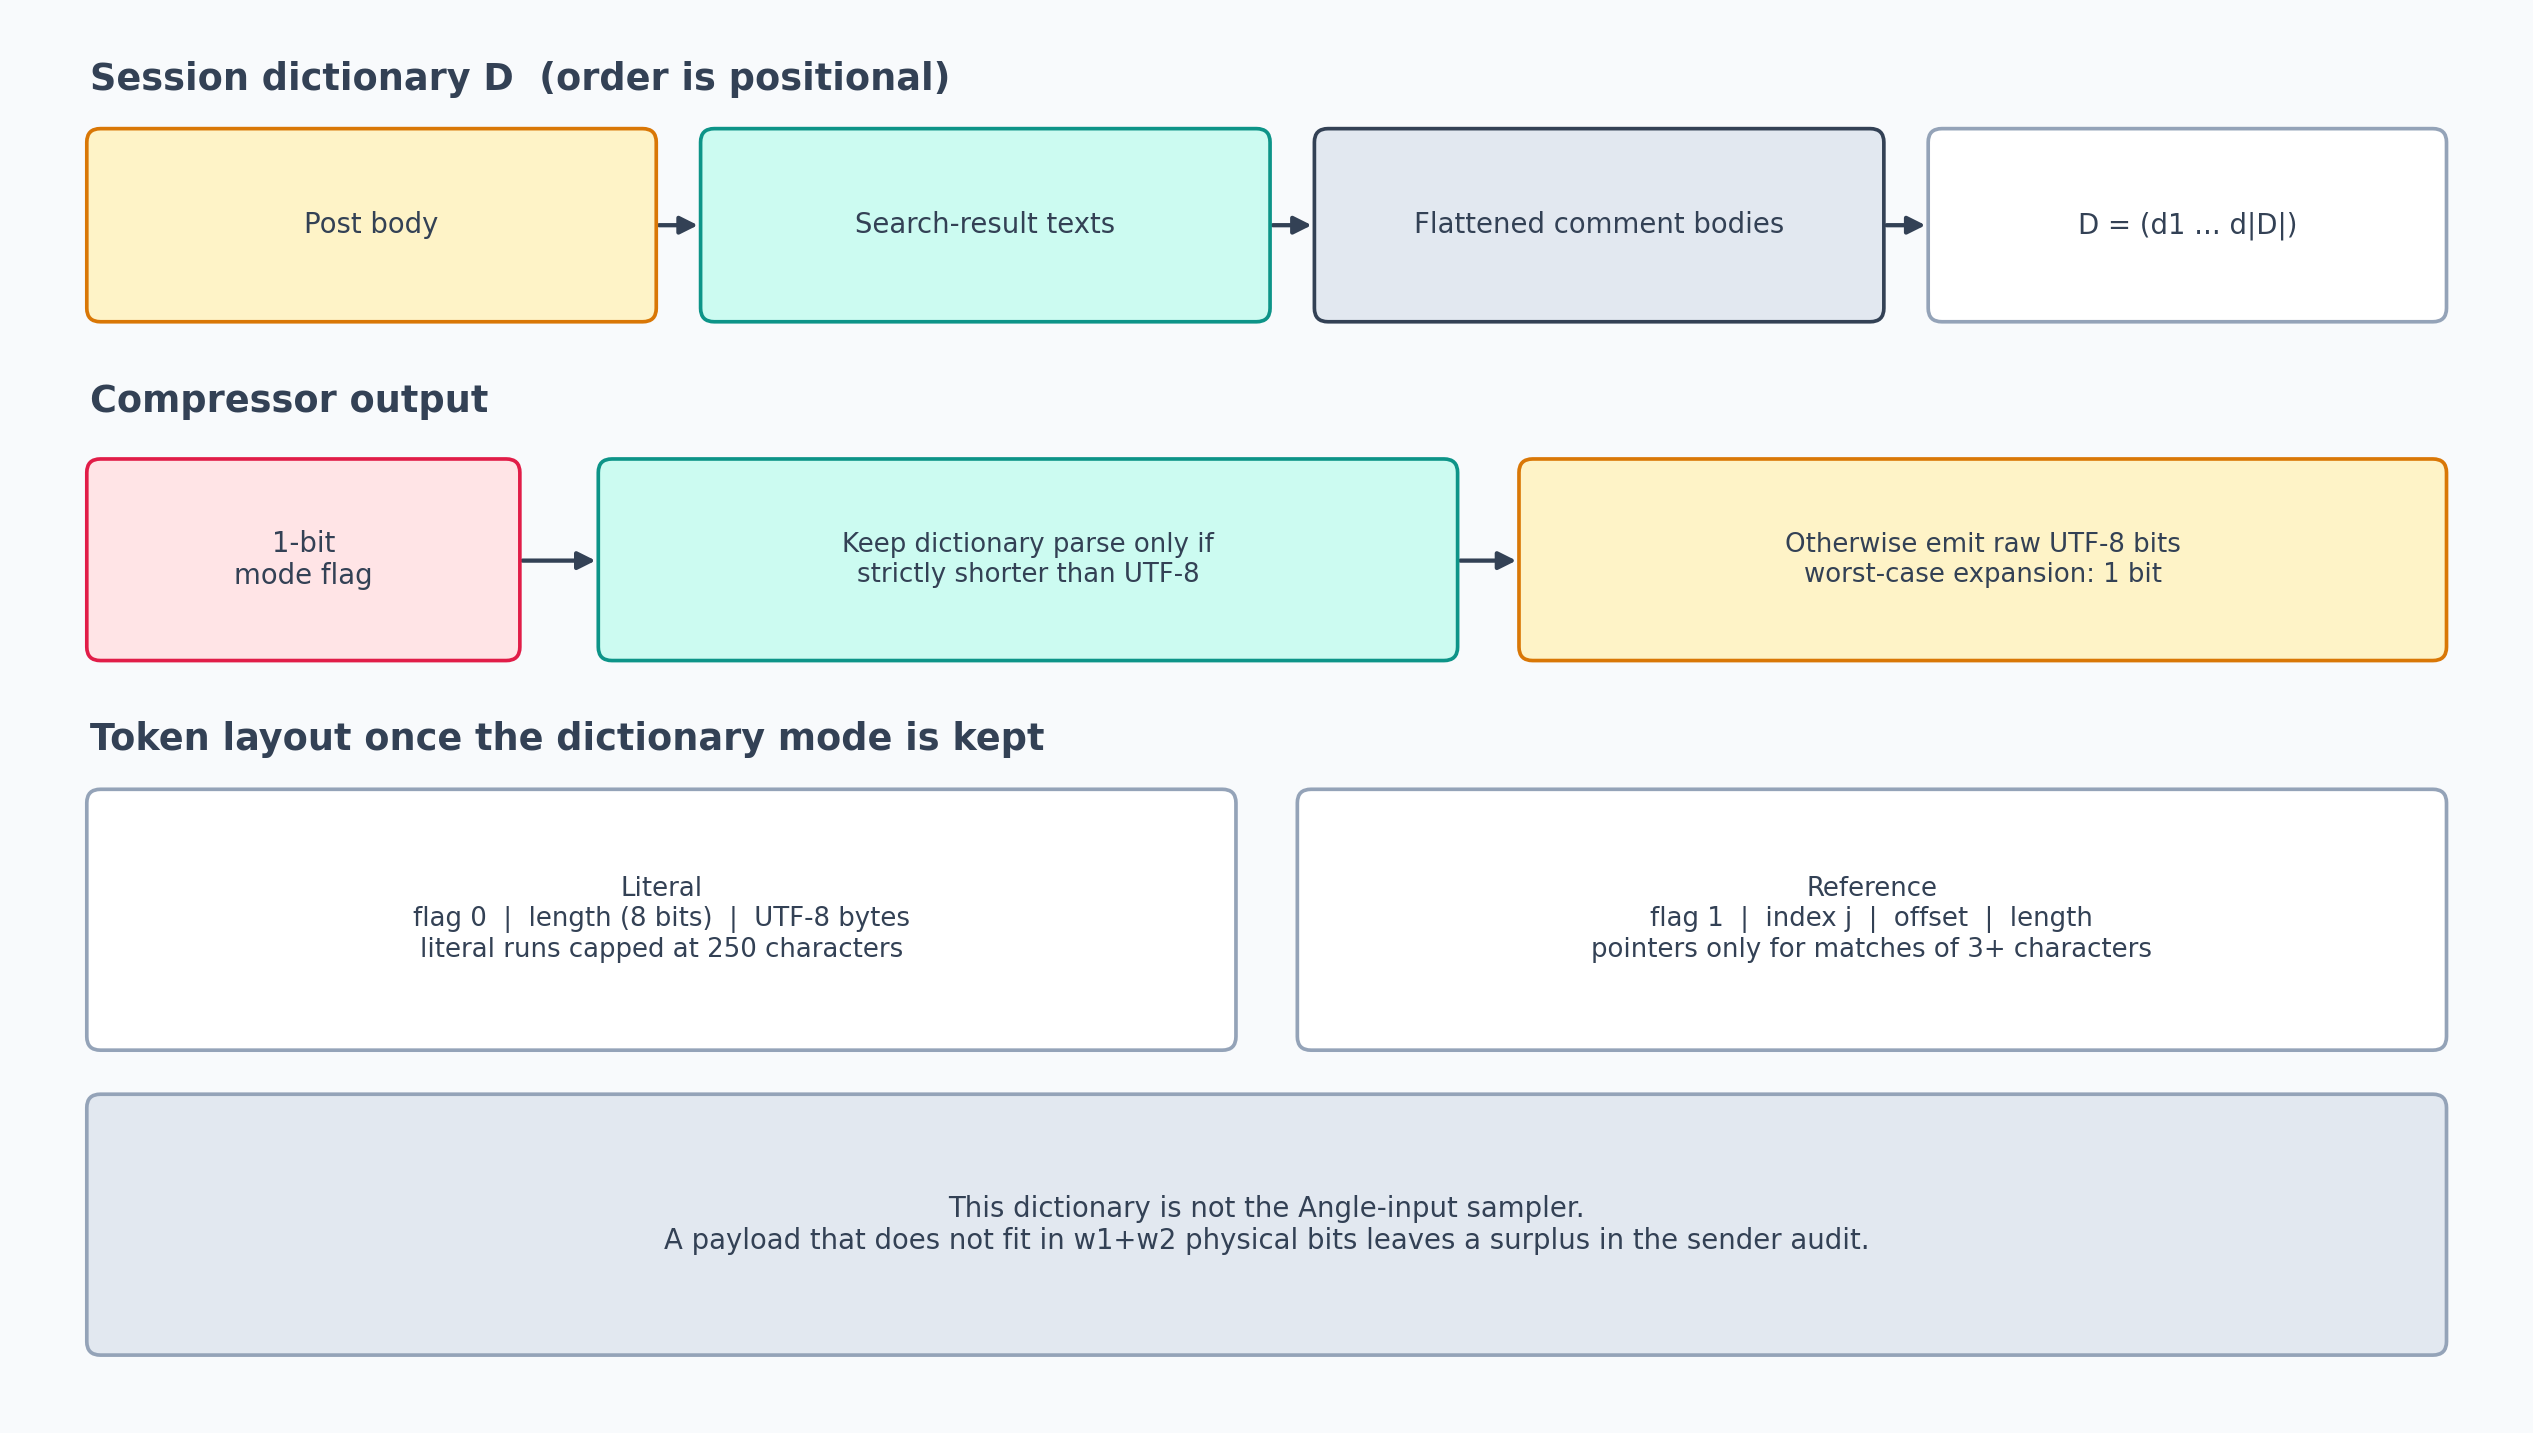
\includegraphics[width=\textwidth,height=0.62\textheight,keepaspectratio]{figures/payload_compression_dp}
	\Description{Schematic of dictionary synthesis from thread and search text, payload segmentation, and choice between literal UTF-8 and dictionary-pointer encoding via a dynamic program.}
	\caption{Payload compression builds a session dictionary from thread and research text, then chooses literal versus dictionary-encoded segments to minimize total bit cost.}
	\label{fig:compression}
\end{figure*}

\subsection{Two-Layer Semantic Embedding Architecture}
Figure~\ref{fig:two-layer} provides the schematic overview of how the two embedding layers split the payload before synthesis.
%
% ------------------------------------------------------------------
% AI IMAGE PROMPT (fig:two-layer) -> figures/two_layer_embedding.(png|pdf)
% ------------------------------------------------------------------
% FORMAT: Wide composite (figure*), roughly two main panels 50/50 or 55/45.
% LEFT PANEL "Layer 1 -- spatial embedding": Tree graph under a root "POST". Draw 2 levels
%   of comments as nodes (circles or cards), children connected with lines. Overlay small
%   integers 1..n along nodes showing deterministic DFS visit order (not post dates). One
%   node with thick amber ring + label "Selected reply parent (index k)". Footnote-style
%   equation text as readable typography: w_1 = ceil(log2(n+1)) and note "index 0 = top-level
%   reply to post". Small legend "Flattened order fixes Alice/Bob agreement".
% RIGHT PANEL "Layer 2 -- shared angle set": Vertical numbered list 0..N-1 (show ~8 rows, ellipsis
%   ok). Each row: thin gray line of lorem-like placeholder (3--5 words, not real sentences).
%   One row highlighted teal with label "selected angle idx". Show w_2 = log2 N as
%   annotation (typeset properly if model supports).
% CENTER BRIDGE (between panels): Horizontal strip of 0/1 bits (12--20 bits), visually split
%   into left segment feeding Layer 1 (label "w_1 bits") and right segment feeding Layer 2
%   ("w_2 bits"). Arrows from segments into respective panels.
% BOTTOM SPAN (full width): Arrow down to box "LLM synthesis (temperature=0.7)" then three
%   small equal-height cards "Candidate comment A/B/C (JSON array)". Emphasize generation,
%   not decoding.
% CONSISTENCY: Match token-vs-intent figure styling (colors, corner radius).
% NEGATIVE PROMPT: binary exploding, matrix code, neural network brain, unreadable tiny math,
%   actual Reddit usernames or vote counts.
% ------------------------------------------------------------------

\begin{figure*}[t]
	\centering
	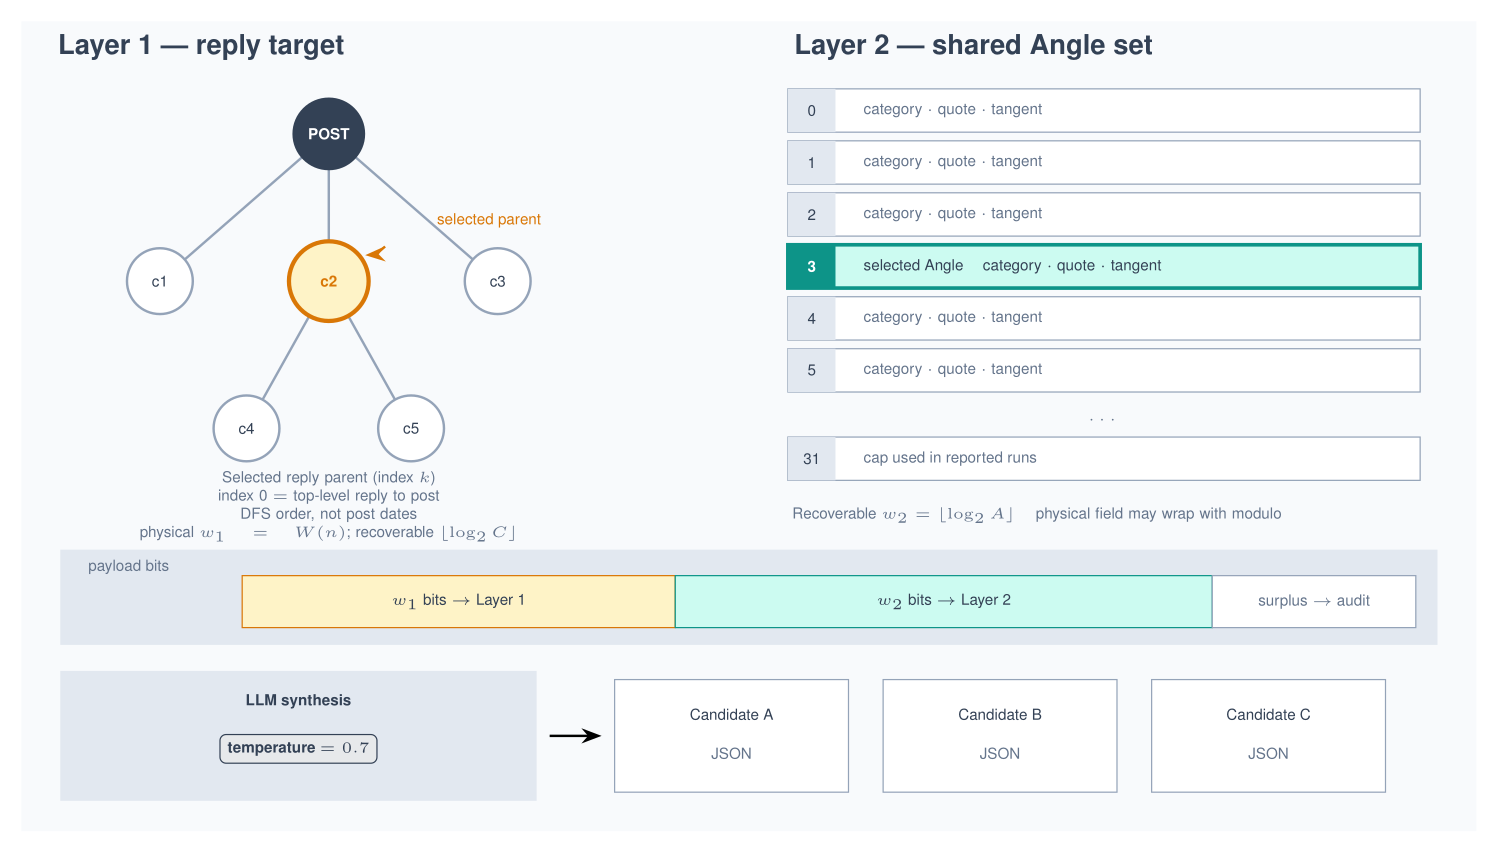
\includegraphics[width=\textwidth,height=0.65\textheight,keepaspectratio]{figures/two_layer_embedding}
	\Description{Two-panel diagram: left, spatial embedding selects a reply parent in a flattened comment tree; right, intent embedding selects an index from a shared angle set; payload bits split across both layers before LLM synthesis.}
	\caption{Two-layer embedding: Layer 1 selects reply placement in a deterministically flattened thread; Layer 2 selects an Angle from a shared, deterministically reconstructed angle set; combined bits drive generative synthesis.}
	\label{fig:two-layer}
\end{figure*}

\subsubsection{Layer 1: Spatial Embedding (Reply Targeting)}
\label{sec:layer1}
The primary embedding layer determines the \textit{architectural placement} of the steganographic contribution.
\begin{enumerate}
    \item The system flattens the nested comment tree with a deterministic depth-first walk, so both sender and receiver number the same comments the same way.
    \item Each reply target gets a fixed-width index, but only $\lfloor\log_2 C\rfloor$ bits of it are guaranteed recoverable, where $C$ is the number of selectable targets (Section~\ref{sec:channel-widths} explains why the raw index width is not safe to use directly).
    \item Index 0 is a top-level reply to the post; any other index selects a specific comment, and the receiver reconstructs that comment's full parent chain by walking up the thread.
\end{enumerate}

\subsubsection{Layer 2: Intent-Based Embedding (Angle Selection)}
\label{sec:layer2}
The secondary layer determines the \textit{communicative intent}.
\begin{enumerate}
    \item \textbf{Angle Set Reconstruction:} Using the deterministic preprocessing chain (Section \ref{sec:search_determinism}) and the filtered thread snapshot, both parties regenerate the same ordered list of candidate Angles, each described by a category label, a source quote, and a tangent field (the thematic direction).
    \item \textbf{Dynamic Bit-Mapping:} The flattened list is assigned sequential \texttt{idx} values, so the recoverable width is $\lfloor\log_2 A\rfloor$ bits for $A$ available Angles --- the same physical-versus-recoverable distinction from Section~\ref{sec:channel-widths} applies here, with $A$ in place of $C$.
    \item \textbf{Angle Selection:} The corresponding payload bits are mapped to a specific Angle index. During synthesis, the selected Angle is paired with the reply context and relevant research excerpts to produce a plausible cover reply.
\end{enumerate}

\subsubsection{Channel Widths and Bit Consumption Order}
\label{sec:channel-widths}
Both layers draw from the front of the same compressed stream produced in Section~\ref{sec:compression}: Layer~1 consumes the first $w_1$ bits, Layer~2 the next $w_2$. Two width notions must be distinguished, and conflating them is the most common way to overstate this channel's capacity.

The \textit{physical} widths are the field sizes actually written to the stream. For a thread with $n$ comments there are $C=n+1$ reply targets, indexed $0$ (a top-level reply to the post) through $n$, so $w_1=W(n)$. For $A$ flattened Angles, $w_2=W(A-1)$. When the integer read from the bits exceeds the largest valid choice, the encoder reduces it modulo the choice count; this happens whenever the choice count is not a power of two. Generation therefore always succeeds, but several bit patterns then collapse onto the same observable selection, so those patterns cannot be inverted.

The \textit{recoverable} widths exclude exactly that aliasing: $\lfloor\log_2 C\rfloor$ and $\lfloor\log_2 A\rfloor$. The lossless embedding path enforces this in two steps: it restricts each field's input to its recoverable width, then re-encodes that value at the full physical width before writing it. The result is a bits-to-selection map that is injective by construction. Capacity claims in Section~\ref{sec:evaluation} use these recoverable widths.

Consuming a prefix rather than a self-delimiting unit --- one that states its own length up front --- has two consequences. First, the very first bit Layer~1 reads is the compressor's mode flag, so the two layers depend on the compressor's output, not only on the thread and Angle set. Second, one post carries exactly $w_1+w_2$ \textit{physical} bits (Section~\ref{sec:channel-widths}); a longer payload leaves a surplus, which the encoder reports as unembedded rather than dropping silently. Recovering a payload larger than one post's capacity from a single visible comment therefore relies on sender-side metadata (audit-assisted recovery), and is reported as such in the evaluation. Blind recovery at scale is instead the job of the multi-frame protocol described next.

\subsection{Multi-Frame Transport}
\label{sec:multiframe}
To carry payloads beyond a single post's capacity, the sender splits the bitstream across several frames, where a frame is one reply comment placed under one post (a single post may host more than one frame --- see below).

The payload is first protected as above and then compressed against an \textit{empty} dictionary, which by the fallback rule of Section~\ref{sec:compression} always yields standard mode: a \texttt{0} flag followed by raw UTF-8 bits. Dictionary compression is deliberately not used here, because frames span several posts and no single session dictionary is shared by all of them.

The resulting bits are prefixed with a control header made of two Elias-gamma codes. An Elias-gamma code represents a positive integer as a unary length prefix followed by its binary value, so its size grows with the number it encodes instead of being fixed in advance. The header encodes the frame count $F$ first, then the payload bit length, so the receiver can read off both quantities before reading any payload bits. A fixed-width header was rejected because the header is itself carried by the same scarce selection channel --- it would need to be sized for the worst case even when $F$ is small.

Frames are then assigned to slots: each post contributes up to a configured number of slots, and each slot's size is the recoverable capacity from Section~\ref{sec:channel-widths}. Sizing this is circular: the control header's length depends on the frame count $F$, but how many slots are needed depends on how large that header is. The planner resolves this by searching upward from $F=1$, stopping at the smallest frame count whose first $F$ slots have enough combined capacity for the stream built for that same $F$. The final frame is zero-padded to fill its slot. On the receiving side, the parser rejects any stream whose declared frame count disagrees with the observed one, or whose padding bits are not all zero --- turning a desynchronized read into a clean failure rather than a plausible wrong payload.

The description above assumes a static Angle pool shared by all frames (the \texttt{post-level} sampler). Under the \textit{context-weighted} sampler --- the mode used to produce the results reported in Section~\ref{sec:evaluation} --- the Angle pool instead depends on which parent comment was selected, so the planner works in two stages per frame: it resolves the parent-selection bits first, regenerates the Angle set conditioned on that parent, and only then measures the Angle field width for the remaining bits.

\subsection{Generative Synthesis \& Verification}
Following the selection of the target context and selected Angle, the sender initiates the cover text synthesis process.
\begin{itemize}
    \item \textbf{Synthesis:} A configurable generative language model (run at non-zero temperature) produces a small fixed set of short, thread-appropriate reply candidates as a JSON list of non-empty strings. The prompt conditions on post metadata, the selected comment chain, the selected Angle (tangent), and relevant research excerpts.
    \item \textbf{Verification Loop:} Before the stego-text is committed to the public channel, the sender executes a local \textit{Decoding Simulation} to verify that the generated text remains recoverable.
    \item \textbf{Recursive Refinement:} If the simulation fails to recover the intended Angle, the sender re-executes synthesis without changing the embedding parameters. The non-zero temperature ensures output variation; the retry loop is capped by a fixed attempt budget.
\end{itemize}
Figure~\ref{fig:verify-decode} summarizes sender-side verification and receiver-side recovery.
%
% ------------------------------------------------------------------
% AI IMAGE PROMPT (fig:verify-decode) -> figures/verify_and_decode_flow.(png|pdf)
% ------------------------------------------------------------------
% STRUCTURE: Two horizontal swimlanes separated by dashed lines, labeled left margin
%   "Sender" (top) and "Receiver" (bottom). Use standard flowchart shapes.
% SENDER LANE: Rectangle "Synthesize 3 JSON comments (T=0.7)" -> Diamond "Local decode
%   simulation succeeds?" -> "No" path curves back to synthesis rectangle with side label
%   "retry (same embedding), max 5 attempts". "Yes" path -> Rectangle "Publish to thread".
%   Small note near loop: "nonzero T varies wording".
% RECEIVER LANE: Rounded rectangle "Observe stego comment" -> Rectangle "Embedding model:
%   cosine similarity shortlist" -> sublabel "top 20 angles". -> Rectangle "LLM discriminator
%   (T=0): return index" -> Rectangle "Map to payload bits / handle rank vs index".
%   Side callout in small text: "If LLM returns 1-based rank, map to shortlist; else fallback
%   to top embedding match".
% CONNECTORS: No vertical arrows between lanes except optional dotted "public channel" between
%   "Publish" and "Observe".
% LEGEND: Tiny key for diamond = decision, rectangle = process.
% NEGATIVE PROMPT: UML class diagrams, sequence diagrams with 20 lifelines, crypto keys,
%   blockchain.
% ------------------------------------------------------------------

\begin{figure*}[t]
	\centering
	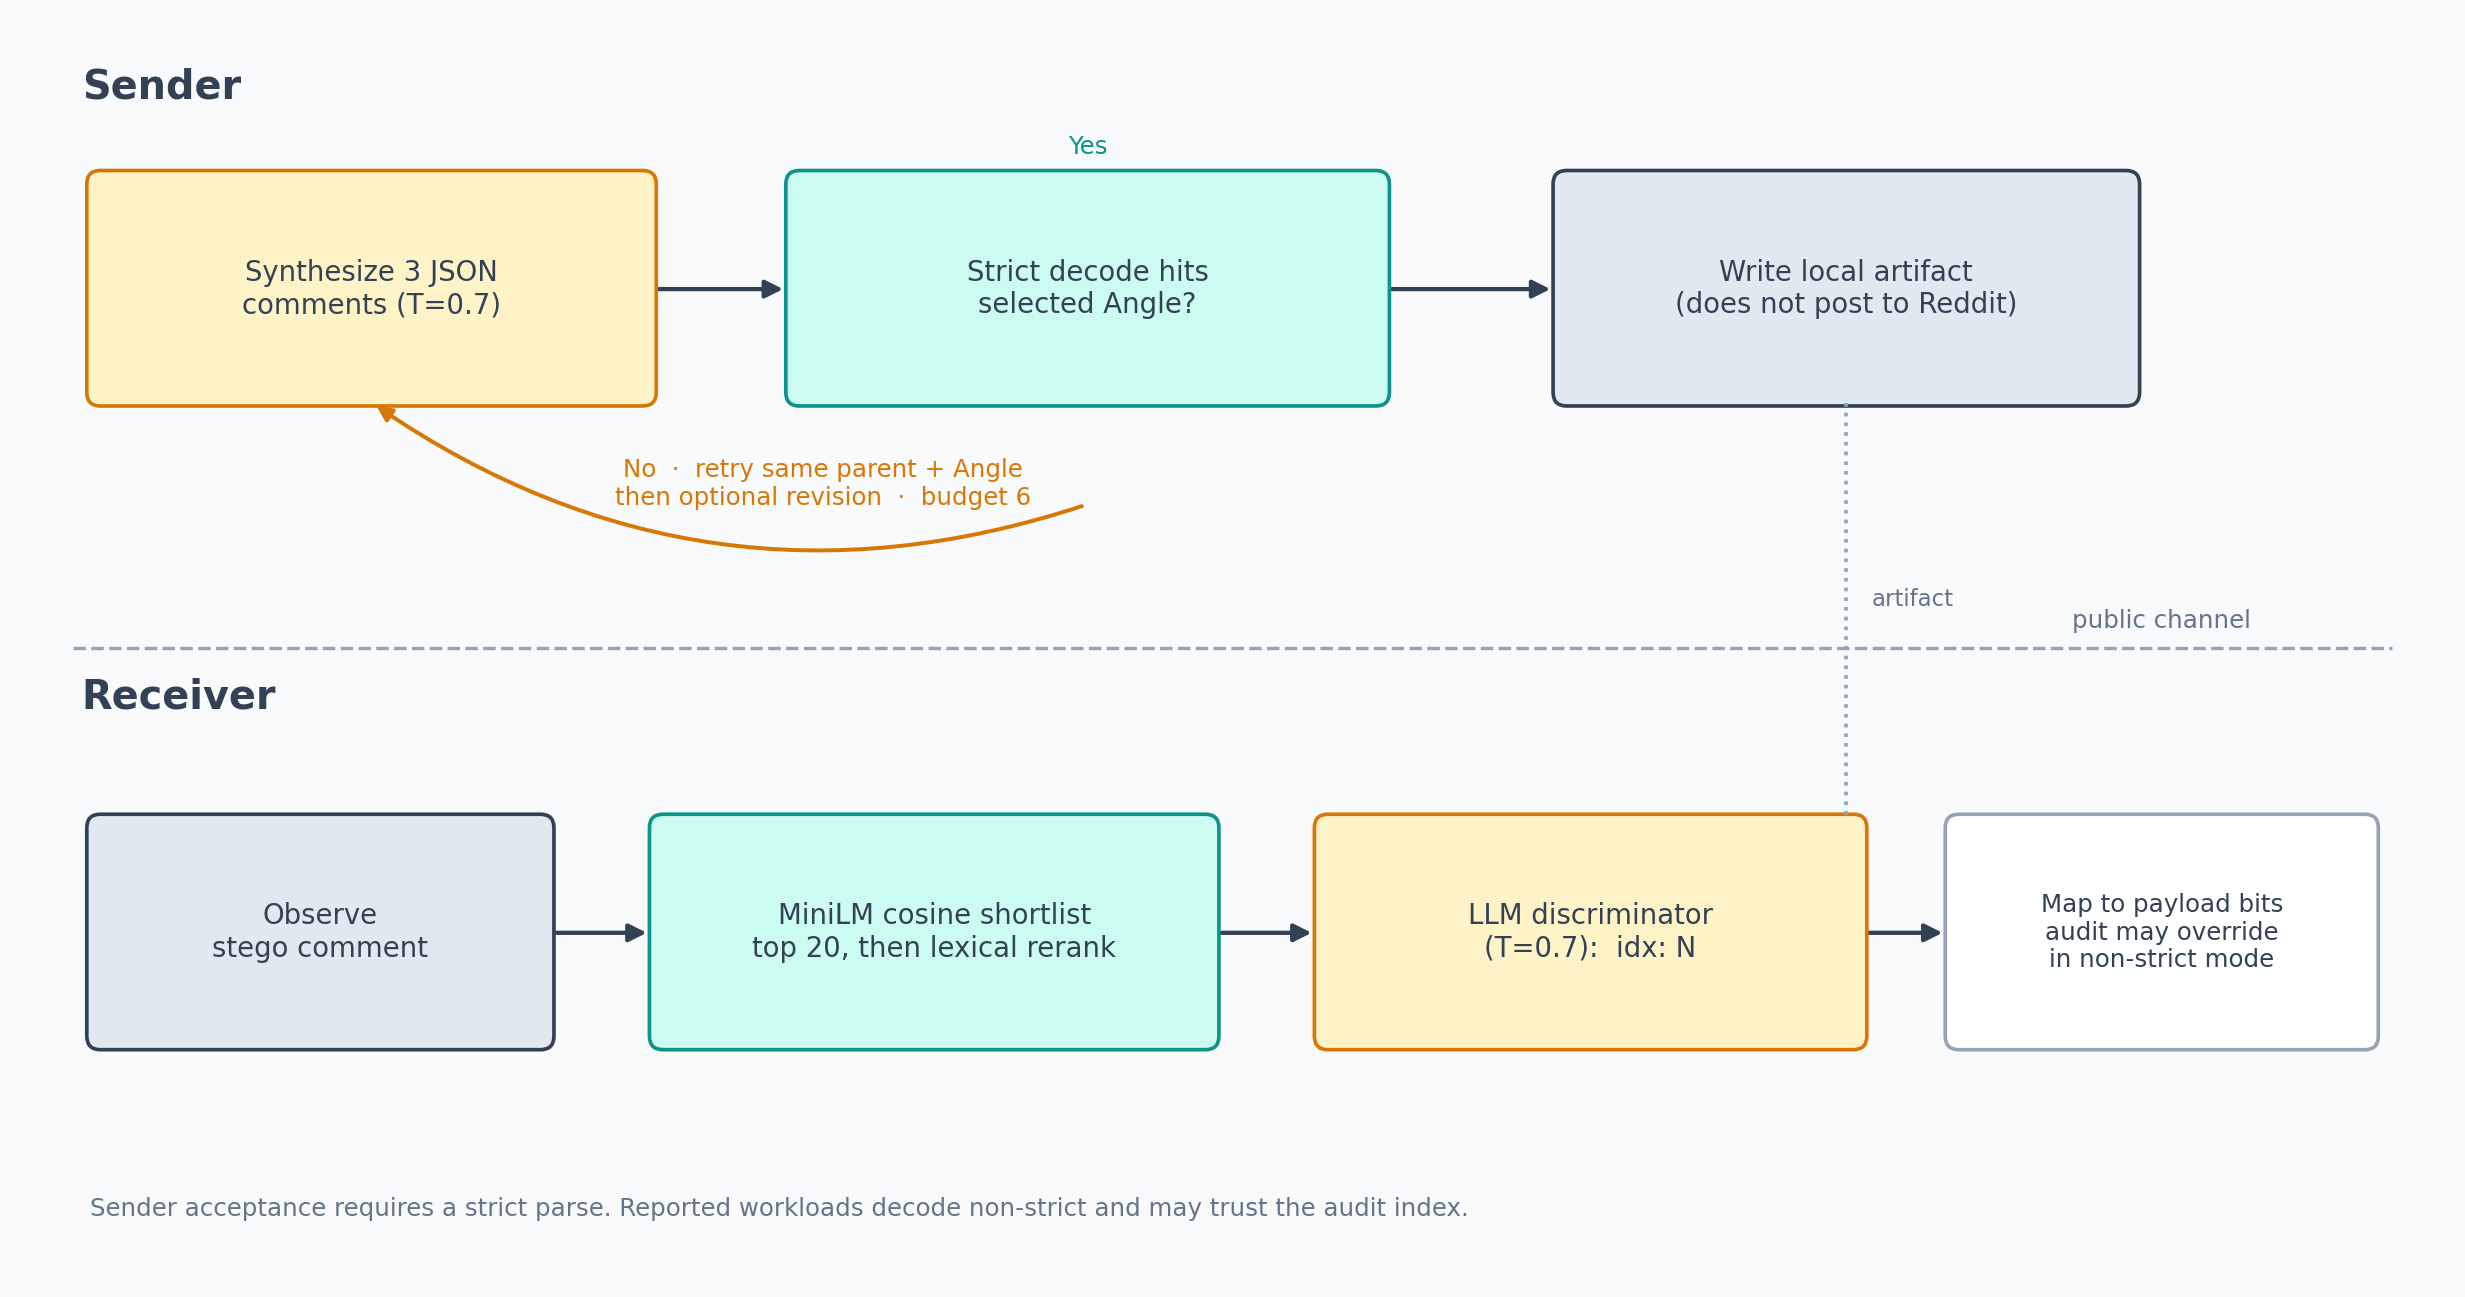
\includegraphics[width=\textwidth,height=0.62\textheight,keepaspectratio]{figures/verify_and_decode_flow}
	\Description{Swimlanes: sender loop synthesizes comments, verifies decode, then publishes; receiver observes the comment, shortlists Angles by semantic similarity, and uses a discriminative prompt to pick the Angle index.}
	\caption{Sender-side verification retries synthesis until decode succeeds; the receiver recovers Layer~2 via semantic shortlisting and a discriminative identification step.}
	\label{fig:verify-decode}
\end{figure*}

\subsection{Decoding \& Intent Recovery}
To recover the hidden intent (Layer 2), the receiver first reconstructs the pre-sender context deterministically, then decodes the Angle selection from the visible reply:
\begin{enumerate}
    \item \textbf{Context Reconstruction:} The receiver locates the candidate stego comment, removes it from the thread, applies the temporal cutoff ($t_{publish} - T_{sync}$), and reruns deterministic preprocessing (URL normalization, research, and angle generation) to reproduce the same ordered Angle list.
    \item \textbf{Semantic Filtering:} A semantic similarity model shortlists the top-$N$ Angles whose text descriptions best match the observed stego reply.
    \item \textbf{Discriminative Identification:} A deterministic identification prompt is executed on the shortlisted candidates to return the most likely Angle index:
          \begin{quote}
              \textit{"Identify the specific Angle from the provided candidates... return the index only."}
          \end{quote}
\end{enumerate}
If the discriminator returns a 1-based rank rather than a raw index, the pipeline maps the rank back to the shortlist; otherwise it falls back to the top semantic match. The decode temperature and shortlist size are configurable, so this stage is not inherently deterministic. Recovery may therefore be pure selection-channel recovery only when the receiver reconstructs the same inputs and decoder contract, or audit-assisted when sender metadata is available. Combined with Layer~1 (reply targeting), the recovered indices reconstruct the selection bits.
\FloatBarrier

\section{Implementation}
\label{sec:implementation}

The runnable pipeline is five stages: data load, research, Angle generation, stego encoding, and decode.
Each stage writes artifacts to disk so later stages can reuse the same corpus and hashes.
Search-term generation and Angle extraction run at \texttt{temperature=0} from the same inputs.
Comment writing and Angle identification do not: both use the shared stego temperature (0.7 on the balanced profile).

\subsection{Pipeline stages}
\begin{itemize}
    \item Data load fetches unresolved URL content and replaces the post body with the extracted text.
    \item Research generates search terms from the post title, body, and URL at temperature 0, trims them to the profile cap (8 on balanced), queries a fixed-shape search backend with fallbacks after Google, drops duplicate links and PDFs, and fetches page text in batches of three. It stores the flat search-results corpus and integrity hashes.
    \item Angle generation flattens the chosen input documents and extracts triplets of category, source quote, and tangent. Long inputs are split into 30k-character segments and batched up to 80k characters by default. If the backend path fails, the pipeline falls back to a direct LLM prompt with the same JSON schema. The reported runs used a context-weighted sampler at this stage, once per post.
    \item Encoding protects and compresses the payload, spends bits on a reply target and an Angle, writes three candidate comments, and keeps a candidate only if a strict local decode hits the selected Angle and a contextuality gate passes.
    \item Decode shortlists Angles with MiniLM cosine similarity, reranks with lexical overlap, and asks for \texttt{idx: N} at the stego temperature. The full reconstruction path can rebuild research and Angles; the reported workloads decode against the sender's already-angled post and pass the audit bitstring.
\end{itemize}
Figure~\ref{fig:impl-pipelines} aligns these stages with the on-disk artifacts.

\subsection{Shared codec}
The bit layer in Sections~\ref{sec:compression}--\ref{sec:multiframe} lives in one module of pure functions.
Dictionary construction for compression, the field-width function $W$, the token grammar, and the physical-versus-recoverable width rules each have one definition there.
The sender and receiver call that module rather than reimplementing it, so round-trip tests can drive the codec with fixtures and no model.

The pipelines around it still own parent lookup, Angle regeneration, semantic search, the discriminator, audit override, and revision.
They are not limited to I/O.

Three configuration choices change the bit layer, so both sides must agree: the payload transform (\texttt{plain}, \texttt{hmac\_xor\_v1}, or \texttt{secure\_compact\_v2}), the pre-shared secret required by the keyed modes, and whether the compressor’s dictionary capacity profile is on.
The sender records the transform in the run audit.
The compressor capacity profile is off by default because dictionary indices are positional.

Table~\ref{tab:token-layout} is the token layout used by the dictionary parse.
A literal is flag \texttt{0}, an 8-bit character length, then UTF-8 bytes.
A reference is flag \texttt{1} plus index, offset, and length fields sized by $W$.
Decoding is sequential: a token’s start depends on where the previous token ended.

\begin{table}[t]
\centering
\caption{Token layout of the compressed payload stream. Every field has a fixed width given the session dictionary $D$, but decoding is sequential: a token's start position depends on where the previous token ended.}
\label{tab:token-layout}
\small
\begin{tabularx}{\columnwidth}{@{}l X l@{}}
\toprule
Token & Field layout & Cost (bits) \\
\midrule
Literal & \texttt{0} $\Vert$ length $\ell$ (8 bits) $\Vert$ UTF-8 bytes & $9+8b$ \\
Reference & \texttt{1} $\Vert$ index $j$ ($W(|D|)$ b) $\Vert$ offset ($W(|d_j|)$ b) $\Vert$ length ($W(L_{\max})$ b) & $1+W(|D|)+W(|d_j|)+W(L_{\max})$ \\
\bottomrule
\end{tabularx}
\end{table}

The single-comment encoder writes physical widths and wraps overflow with modulo.
The multi-frame planner uses the lossless writer that stores only recoverable widths.
% Figure generated by scripts/redraw_live_method_figures.py.

\begin{figure*}[t]
	\centering
	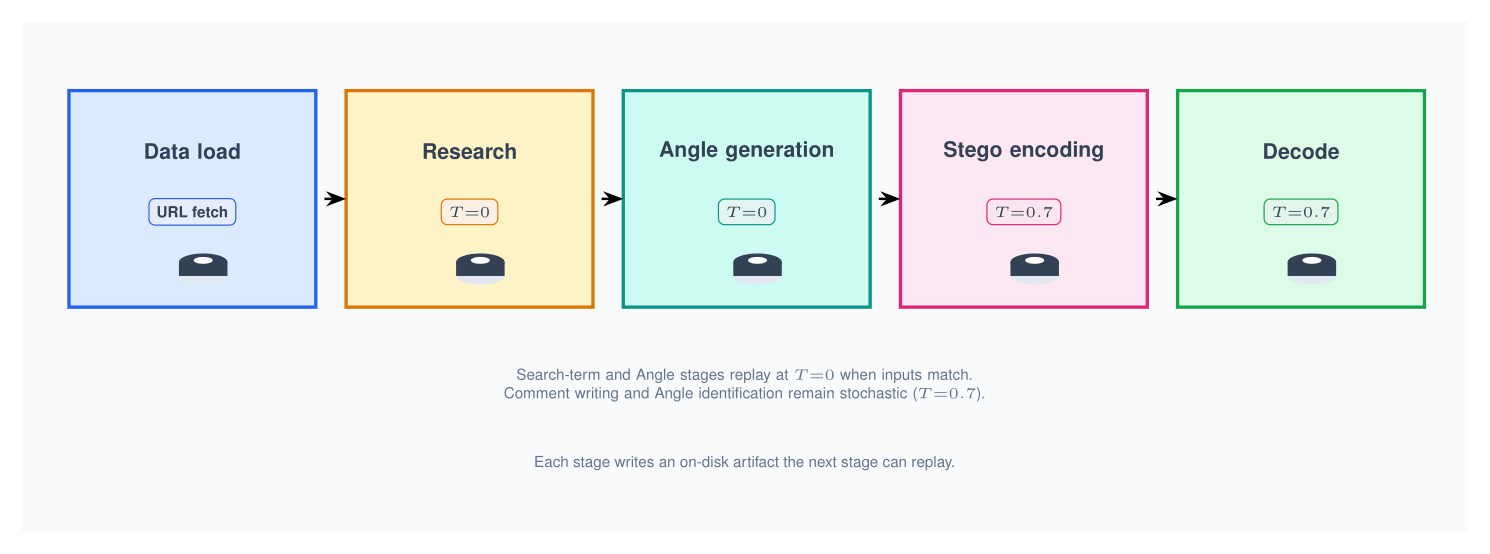
\includegraphics[width=\textwidth,height=0.55\textheight,keepaspectratio]{figures/implementation_pipelines}
	\Description{Block diagram of implementation pipeline stages and on-disk artifacts supporting replay and sender--receiver alignment.}
	\caption{Implementation stages and persisted artifacts. Search-term and Angle stages replay at temperature 0 when the inputs match; comment writing and Angle identification remain stochastic.}
	\label{fig:impl-pipelines}
\end{figure*}

\subsection{Model roles}
Exact model IDs are configuration.
The roles are not:
\begin{itemize}
    \item Search-term generation and Angle extraction run at \texttt{temperature=0} so both parties can rebuild the same lists from the same inputs.
    \item Comment writing runs at nonzero temperature (0.7 on balanced) so retries produce different wording for the same parent and Angle.
    \item Angle identification uses MiniLM cosine similarity, a default shortlist of 20 with lexical rerank, then the same stego temperature for an \texttt{idx: N} prompt. It is not a temperature-0 oracle.
\end{itemize}

\section{Evaluation}
\label{sec:evaluation}

This section reports an artifact-based assessment of the workflow, focusing on (i) embedding capacity of the selection channel, (ii) naturalness and distributional divergence of successful stego samples, and (iii) operational reliability under the sender-side verification loop. We center results on a clean run artifact (\texttt{run\_id} \texttt{20260509T203344Z}, directory \texttt{metrics/e2e\_runs/fresh\_metrics\_200\_20260509T233342Z}) and explicitly separate generation/decode failures from infrastructure errors.

\subsection{Capacity Analysis}
The channel capacity of Layer~2 is fundamentally dependent on the size of the shared, deterministically reconstructed angle set. If the reconstructed set contains $N$ Angles, then Layer~2 contributes $\log_2 N$ bits per message instance (rounded up to an integer bit-width in the implementation). In practice, broader threads and richer research corpora tend to yield larger and more diverse angle sets than narrowly constrained topics, increasing available capacity.

\subsection{Perceptual \& Statistical Imperceptibility}
Imperceptibility is evaluated through the dual lenses of semantic coherence and contextual integration. Unlike traditional steganographic methodologies that risk producing disjointed or statistically anomalous text, our intent-based approach aims to ensure that each stego contribution maintains a clear thematic alignment with the surrounding discourse. In this work we report GPT-2 perplexity and word-unigram KL/JSD as coarse statistical proxies, noting that these metrics do not fully capture long-context semantic quality \cite{wang2022perplexity} and do not replace dedicated steganalysis benchmarks.

Table~\ref{tab:method-metrics} summarizes perplexity (GPT-2) and word-unigram divergence against two baselines: the matched primary post and a global comment corpus. Values are computed over the successful, receiver-validated stego samples produced in run \texttt{20260509T203344Z} (\texttt{requested}=200, \texttt{succeeded}=183).

\begin{table}[t]
	\centering
	\caption{Perplexity and distribution divergence for stego comments (GPT-2 PPL; KL/JSD on word unigrams).}
	\label{tab:method-metrics}
	\small
	\begin{tabularx}{\columnwidth}{@{}l l X c X@{}}
		\toprule
		Category & Metric & Baseline / context & Mean & Range (min / max) \\
		\midrule
		Perplexity & PPL (GPT-2) & 183 successful stego strings & $\approx 142.3$ & 22.8 -- 653.8 \\
		\midrule
		Divergence & KL & Matched primary post & $\approx 9.24$ & --- \\
		Divergence & KL & Global comment corpus & $\approx 6.50$ & --- \\
		Divergence & JSD & Matched primary post & $\approx 0.590$ & --- \\
		Divergence & JSD & Global comment corpus & $\approx 0.588$ & --- \\
		\bottomrule
	\end{tabularx}
\end{table}

\paragraph{Definitions.}
Perplexity is computed from average per-token log-probability,
$2^{-\frac{1}{n} \sum_{i=1}^{n} \log_2 P(x_i \mid x_{<i})}$:
lower PPL indicates more natural continuations under the model; higher PPL indicates surprising or awkward text.
The observed maximum ($\sim$654) likely reflects a small number of pathological samples that are highly unnatural to GPT-2.

Kullback--Leibler (KL) divergence compares stego word unigrams $P_S$ to a baseline $P_C$ via
$\sum_w p_{\text{stego}}(w) \log \frac{p_{\text{stego}}(w)}{p_{\text{baseline}}(w)}$;
lower KL indicates closer statistical match to the baseline.
KL being lower against the global corpus than against the matched post suggests stego wording drifts toward generic phrasing rather than thread-specific vocabulary.

Jensen--Shannon divergence (JSD) is the symmetric, bounded counterpart,
$D_{\mathrm{JS}}(P_C \,\|\, P_S) = \frac{1}{2} D_{\mathrm{KL}}\bigl(P_C \,\|\, \frac{P_C + P_S}{2}\bigr) + \frac{1}{2} D_{\mathrm{KL}}\bigl(P_S \,\|\, \frac{P_C + P_S}{2}\bigr)$,
often used to upper-bound distinguishability from the true language distribution.
Word pairs absent from one side of the comparison are handled with Laplace-style smoothing (e.g., $\alpha = 10^{-6}$) so KL and JSD remain well defined.

Table~\ref{tab:metrics-vs-literature} contrasts these means with representative values from related work (exact comparability varies by corpus and tokenization).
Table~\ref{tab:slr-metrics-comparison} uses the same column layout as our systematic-review extraction sheet: paper, model, corpus, reported metrics, and context tags, with our row listed first for side-by-side reading.

\begin{landscape}
	\footnotesize
	\setlength{\tabcolsep}{4pt}
	\begin{longtable}{@{}p{2.05cm}p{2.35cm}cp{1.85cm}p{5.35cm}p{1.45cm}p{1.55cm}p{1.95cm}@{}}
		\caption{This work versus prior papers (SLR-style summary; metrics are as stated in each paper and may use different models, tokenizations, and baselines).}
		\label{tab:slr-metrics-comparison} \\
		\toprule
		Paper & LLM & Yr. & Dataset & Result & Ctx.\ aware & Cat.\ ctx.\ & Repr.\ ctx.\ \\
		\midrule
		\endfirsthead
		\multicolumn{8}{c}{\tablename\ \thetable{}---continued from previous page} \\
		\toprule
		Paper & LLM & Yr. & Dataset & Result & Ctx.\ aware & Cat.\ ctx.\ & Repr.\ ctx.\ \\
		\midrule
		\endhead
		\midrule
		\multicolumn{8}{r}{\emph{Continued on next page}} \\
		\endfoot
		\bottomrule
		\endlastfoot
		This work & Configurable black-box LLMs (deterministic decode; stochastic synthesis); GPT-2 for PPL & 2026 & Threaded forum posts; run \texttt{20260509T203344Z} (183 successes) & PPL $\approx 142.3$; KL 6.50 (global) / 9.24 (matched); JSD 0.588 (global) / 0.590 (matched) & explicit & social thread & selection channel (reply + angle) \\
		\midrule
		VAE-Stega \cite{yang2020vae} & BERT--LSTM; LSTM--LSTM (from scratch) & 2020 & Twitter (2.6M sents.); IMDB (1.2M sents.) & PPL 28.879; $\Delta$MP 0.242; KLD 3.302; JSD 10.411; Acc 0.600 & non-explicit & pre-text & text \\
		General MLM RH \cite{zheng2022general} & BERT-base & 2022 & BookCorpus & BPW 0.5335; F1 0.9402; PPL 134.22 & non-explicit & pre-text & text \\
		Co-Stega \cite{liao2024co} & Llama-2-7B/13B-chat; fine-tuned GPT-2 & 2024 & Twitter; tweet data for fine-tuning & SR1 60.87\%; SR2 98.55\%; cap.\ 44.91 bit; BPW 2.31; PPL 16.75; SimCSE 0.69 & explicit & social media & text \\
		Joint BERT--GAT \cite{ding2023joint} & LSTM+attn.; GAT; BERT MLM & 2023 & OPUS & PPL 13.917; KLD 2.904; SIM 0.812; ER 0.365; best Acc 0.575 & explicit & pre-text & text \\
		Discop \cite{ding2023discop} & GPT-2 & 2023 & IMDB & $p{=}1.00$; ave.\ KLD 0; max KLD 0; cap.\ 5.76 bit/token; PPL $\approx 42$ (stego quality in paper) & non-explicit & tuning + pretext & text \\
		LLM generative stego \cite{wu2024generative} & Any LLM (e.g., GPT-4 in eval.) & 2024 & [not specified] & len.\ 13.3 words; BPW 5.93; PPL 165.76; SS 0.5881; BiLSTM Acc 49.2\% & explicit & [varies] & [varies] \\
		Zero-shot ling.\ stego \cite{lin2024zero} & LLaMA2-Chat-7B; GPT-2 for baselines & 2024 & IMDB; Twitter & PPL 8.81; JSD$_\text{full}$ $17.9{\times}10^{-2}$; JSD$_\text{half}$ $16.86{\times}10^{-2}$; JSD$_\text{zero}$ $13.40{\times}10^{-2}$ & explicit & zero-shot + prompt & text \\
		Provably secure disamb.\ \cite{qi2024provably} & LLaMA2-7B; Baichuan2-7B & 2024 & IMDb (EN/ZH samples) & err.\ 0\%; ave.\ KLD 0; ave.\ PPL 3.19 (EN), 7.49 (ZH); cap.\ 1.03--3.05 bit/token & non-explicit & pretext & text \\
		Hi-Stega \cite{wang2023hi} & GPT-2 & 2024 & Yahoo! News (titles/bodies/comments) & PPL 109.60; MAUVE 0.2051; ER2 10.42; $\Delta$cosine 0.0088; $\Delta$SimCSE 0.0191 & explicit & social media & text \\
	\end{longtable}
\end{landscape}

\begin{table}[t]
	\centering
	\caption{Comparison of measured means to illustrative values from the literature.}
	\label{tab:metrics-vs-literature}
	\footnotesize
	\begin{tabularx}{\columnwidth}{@{}l c X@{}}
		\toprule
		Metric & Ours (mean) & Source reference and context \\
		\midrule
		PPL & 142.3 & 134.11 (human mean), VAE-Stega / IMDB training baseline. \\
		PPL & & 20.92 (RNN-Stega), VAE-Stega RNN at 1.0 bpw. \\
		PPL & & 165.76 (LLM-Stega), black-box generation with GPT-4. \\
		PPL & & 42.23 (Discop), stego quality with GPT-2. \\
		\midrule
		KL & 6.50--9.24 & 19.51 (RNN-Stega), VAE-Stega RNN on IMDB. \\
		KL & & 0.045 (Meteor), high-entropy English sampling. \\
		KL & & 0.00 (Discop), distribution-matching stego. \\
		\midrule
		JSD & 0.588--0.590 & 14.48 (RNN-Stega), VAE-Stega RNN on IMDB. \\
		JSD & & 0.18 (Zero-shot LLM), in-context learning ($17.9 \times 10^{-2}$). \\
		\bottomrule
	\end{tabularx}
\end{table}

\paragraph{Reading the comparison.}
Mean PPL ($\approx 142.3$) is of similar scale to the human-text average reported for VAE-Stega (134.11) and lower than a cited black-box LLM-Stega reference (165.76), i.e., within a plausible range for non-adversarial generated forum-style text when evaluated under GPT-2.
KL (6.50--9.24) is much smaller than the RNN-Stega IMDB figure (19.51), indicating stronger unigram-level alignment with the chosen baselines than older recurrent generators, but larger than methods that tightly match a model distribution (Meteor, Discop), which operate at token level or with provable distribution matching.
JSD (0.588--0.590) exceeds the cited zero-shot LLM value (0.18), so the stego text retains a more distinct unigram signature than that reference.
Finally, lower KL to the global corpus than to the matched post parallels a known pattern: as surface quality is pushed, text may move toward background forum language and away from idiosyncratic thread-specific vocabulary.

\subsection{System Robustness \& Recovery Rate}
The sender-side verification loop improves operational reliability by rejecting candidates that do not decode back to the selected Angle. In run \texttt{20260509T203344Z} (\texttt{requested}=200), the pipeline produced 183 successful, receiver-validated samples and 17 failures after exhausting the retry budget. The primary failure modes were (i) decoding validation failures (10/17) and (ii) malformed synthesis output that did not match the required JSON schema (7/17). These failures highlight that reliability is primarily limited by the ability to synthesize a decodable witness under stochastic generation, rather than by payload recovery after validation.

\subsection{Resistance to Automated Steganalysis}
The design objective of the framework is to reduce semantic and pragmatic anomalies by conditioning synthesis on the full thread context and by encoding information in conversational decisions (reply targeting and Angle selection) rather than local token artifacts. We therefore expect detection to require thread-level pragmatic reasoning rather than relying solely on token-level distribution cues \cite{Wang_2023}. A dedicated steganalysis benchmark evaluation is left to future work; here we limit claims to the measured distributional and operational metrics reported above.

\section{Conclusion}
\label{sec:conclusion}

This work hides a payload in a threaded discussion by choosing a reply target and an Angle, then asking an LLM to write an ordinary comment.
Capacity is whatever those two lists uniquely decode.
The design does not insert bits into next-token sampling, and it does not need white-box logits.

An independent LLM-judge run on 244 unique-output pairs found ZLG harder to pick in a same-thread lineup (28.3\% versus 51.6\% standout detection) and our method higher on register-fit (3.193 versus 2.791, paired sign-test $p=0.00374$).
The source campaign succeeded on 2{,}543 of 4{,}044 LUCID attempts, all with audit-assisted recovery.
A historical 2026-07-30 configuration, post-clustered over 100 posts, had recoverable capacity 16.00 versus 15.14 bits/comment and GPT-2 perplexity 53.70 versus 68.15, with 554 of 627 project-side attempts succeeding.
Those two artifacts answer different questions.
Neither is a blind, capacity-matched ranking, and neither establishes resistance to an adaptive steganalyst.
Future work should freeze a symmetric manifest, score GPT-2 and divergence on that freeze, decode without sender audit files, and test dedicated steganalysis and editing attacks.


\bibliographystyle{unsrtnat}
\bibliography{references/bibliography}

\end{document}
